%
% main.tex -- Paper zum Thema <nerven>
%
% (c) 2020 Autor, OST Ostschweizer Fachhochschule
%
% !TEX root = ../../buch.tex
% !TEX encoding = UTF-8
%
\chapter{Nervenzellen\label{chapter:nerven}}
\kopflinks{Nervenzellen}
\begin{refsection}
\chapterauthor{Tobias Zuber und Dino Ramcilovic}
\section{Einleitung}

Die Informationsübertragung in unserem Körper wird vom Nervensystem übernommen.
Dies beinhaltet zum Beispiel das vermitteln von Reizen, welche die Augen oder Ohren aufgenommen haben,
an das Gehirn und das Senden von Befehlen vom Gehirn an die Muskeln.
Das Nervensystem besteht aus Nervernzellen, welche elektrische Signale generieren, von anderen Zellen aufnehmen und weiterleiten können.
Die Signale werden so von einer Zelle zur nächsten Zelle weitergeleitet, bis das Signal am Zielpunkt ist.
\subsection{Biologische Grundlagen}
In Abbildung \ref{fig:Aufbau Nervenzelle} ist der Aufbau einer Nervenzelle ersichtlich. 
\begin{figure}[h]
    \centering
    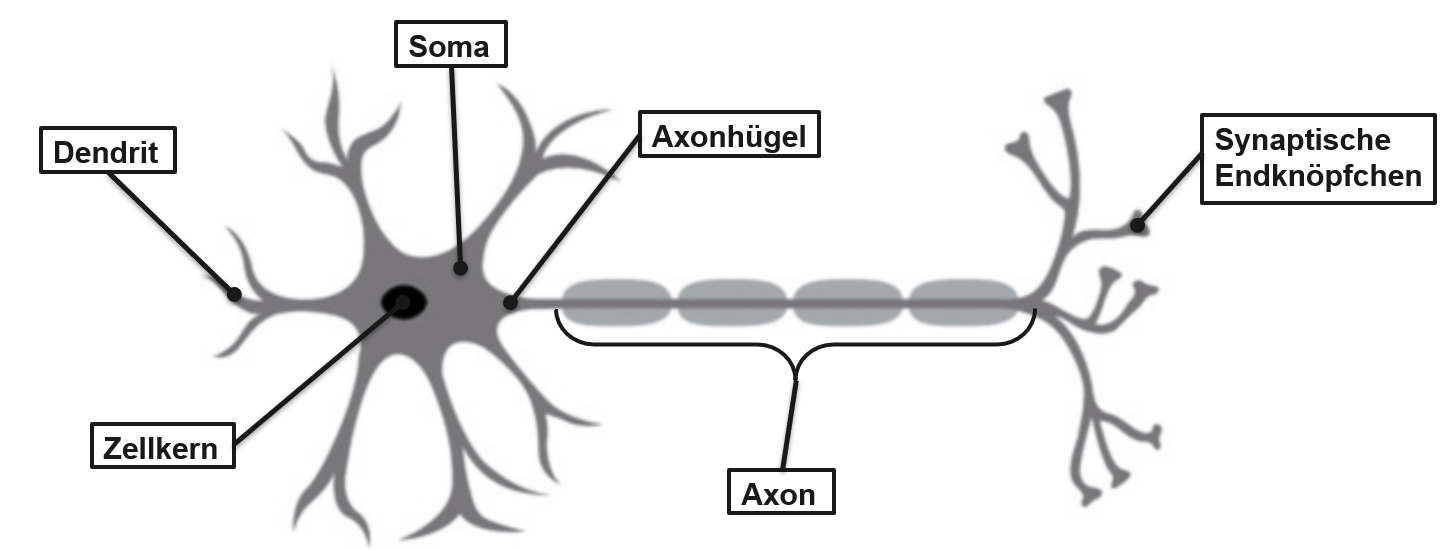
\includegraphics[width=\textwidth]{papers/nerven/Bilder/NervenAufbau2.png}
    \caption{Aufbau Nervenzelle \cite{nerven:rosadu}}
    \label{fig:Aufbau Nervenzelle}
\end{figure}

Die Dendriten empfangen Signale. 
Im Axonhügel im Soma werden basierend auf den empfangenen Singalen elektrische Impulse erzeugt und mithilfe des Axons übertragen.
Die Synapsen sind mit der nächsten Zelle verknüpft und so wird das Signal immer weitergeleitet.

\subsection{Aktionspotential}
Die Nervenzelle besitzt für das Erzeugen von elektrischen Impulsen, das von den empfangenen Signalen bestimmt wird ein Interessantes Verhalten.
Um zu verhindern, dass im Axonhügel ungewollte elektrische Impulse entstehen, gibt es einen Spannungsschwellenwert,
den das empfangene Signal überschreiten muss.
Bei Signalen mit zu kleiner Spannung, wird dieses Signal sofort stark gedämpft und führt auch zu keinem elektrischen Impuls.
Wenn der Schwellenwert jedoch vom empfangenen Signal überschritten wird, gibt es sofort einen grossen elektrischen Impuls,
der entlang des Axons weitergeleitet wird. 
Diesen elektrischen Impuls nennt man Aktionspotential.
\begin{figure}[h]
    \centering
    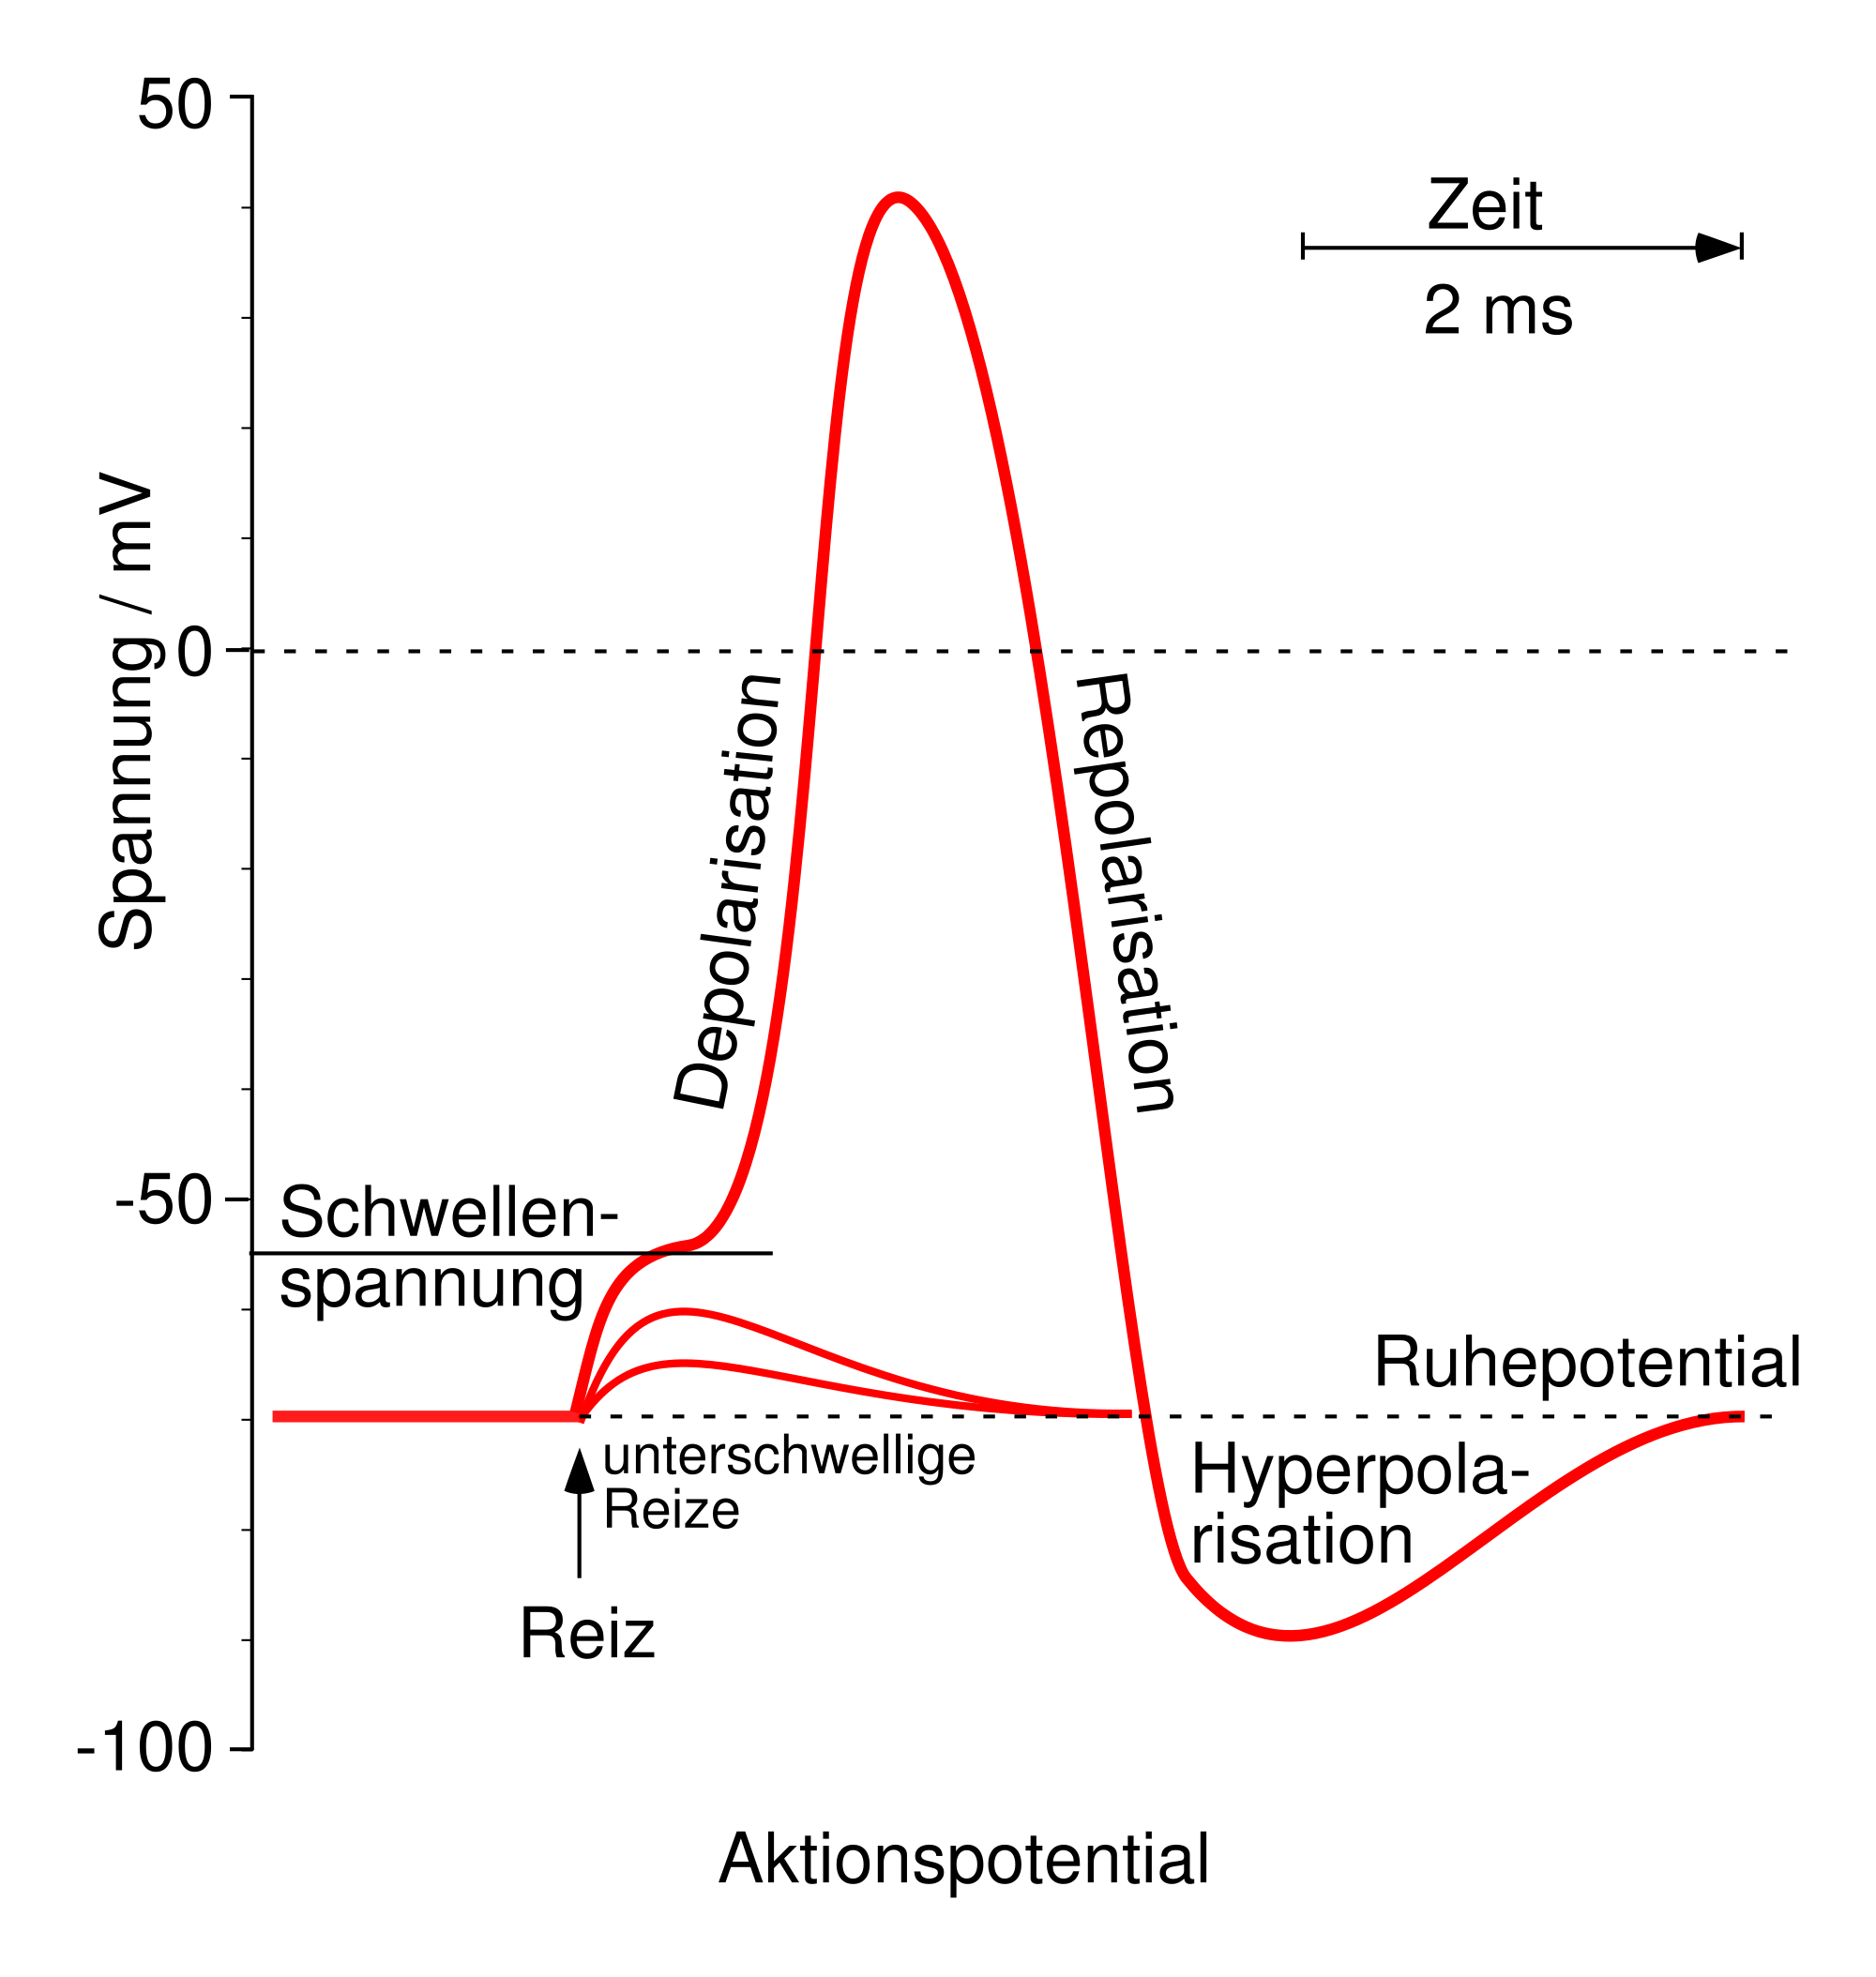
\includegraphics[width=0.8\textwidth]{papers/nerven/Bilder/Aktionspotential.png}
    \caption{Aktionspotential \cite{nerven:JohnEcclesAlanHodgkinAndrewHuxley.}}
    \label{fig:Aktionspotential}
\end{figure}

In Abbildung \ref{fig:Aktionspotential} ist ersichtlich, wie ein Aktionspotential entsteht und schnell wieder abklingt.
Dabei besitzt diese Nervenzelle eine Ruhespannung von $-70$ Millivolt und einen Spannungsschwellenwert von $-50$ Millivolt.
Wenn die Nervenzelle einen Reiz, in Form eines elektrischen Signales erhält, wird eine Entscheidung getroffen. 
Ist die Spannung des Reizes kleiner als der Spannungsschwellenwert, wird dies als unterschwelliger Reiz bezeichnet und klingt sofort ab.
Ist die Spannung jedoch grösser, kommt das Aktionspotential in die Depolarisationsphase und steigt bis auf 40 Millivolt.
Sobald das Aktionspotential diese maximale Spannung erreicht, beginnt die Repolarisationsphase.
Dies bedeutet, die Spannung des Aktionspotentials nimmt schnell wieder ab und wird mit $-70$ Millivolt noch kleiner als die Ruhespannung.
In der Hyperpolarisationsphase beruhigt sich das Aktionspotential wieder und nimmt die Ruhespannung von $-50$ Millivolt an.
Dieser Ablauf des Spannungsimpulses des geschieht in wenigen Millisekunden 
\cite{nerven:InaLammers.31.08.2015}.

\subsection{Biologische Vorgänge}
Um dieses Aktionspotential an einer Nervenzelle verstehen zu können, muss die Zellwand betrachtet werden. 
Das Aktionspotential wird durch das Membranpotential beschrieben, dies ist die Ladungsdifferenz zwischen dem Intra- und
Extrazellulärraum.
In Abbildung \ref{fig:Ruhezustand} ist ein Modell der Zellwand, wenn die Nervenzelle im Ruhezustand ist, dargestellt.
\begin{figure}[h]
    \centering
    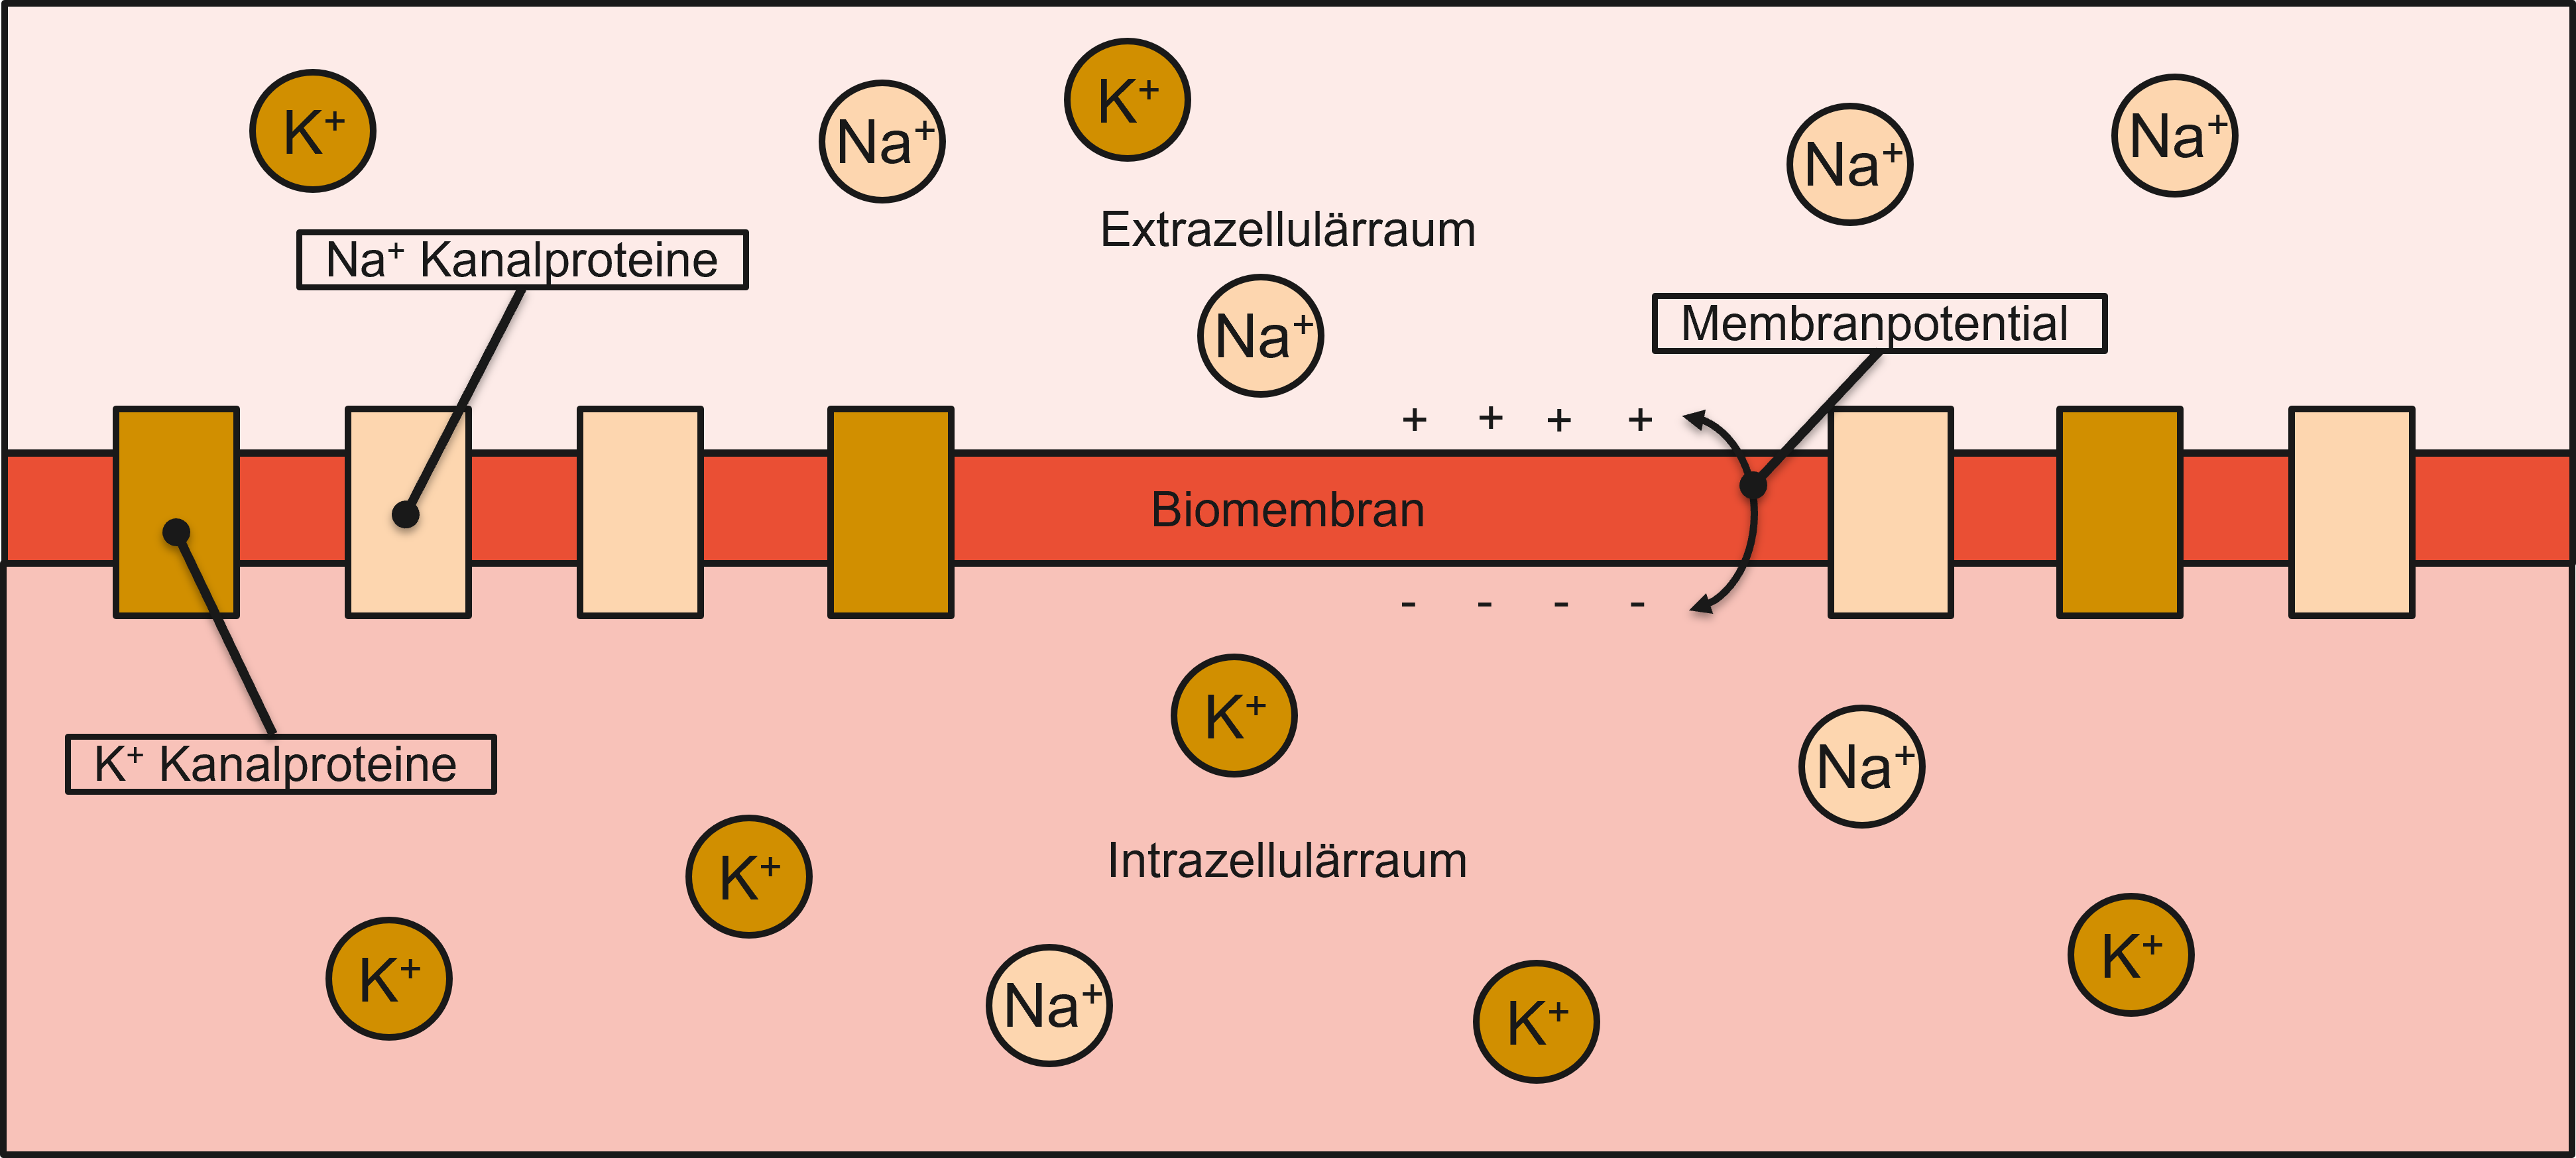
\includegraphics[width=\textwidth]{papers/nerven/Bilder/Vorgang1.png}
    \caption{Ruhezustand: Im Zellinneren tritt eine grössere Kaliumionenkonzentration als im Zelläusseren auf.}
    \label{fig:Ruhezustand}
\end{figure}

Die Ladung von Zellinnerem und Zelläusserem wird durch die Verteilung von positiv geladenen Ionen gesteuert.
Die dafür wichtigsten Ionen sind Kalium- und Natriumionen. 
Eine sogenannte Ionenpumpe ermöglicht, dass sich im Ruhezustand der Zelle mehr Kaliumionen im Zellinneren und mehr
Natriumionen im Zelläusseren befinden.
Da Kaliumionen eine grössere Ladung als Natriumionen besitzen, ergibt sich so das negative Membranpotential von $-70$
Millivolt.
Die Zellwand besteht aus einer Biomembran, die für Moleküle und Ionen undurchlässig ist.
In der Zellwand befinden sich jedoch Kanalproteine, die bei der richtigen Anregung spezifische Ionen durch die
Biomembran transportieren können.

Wenn die Nervenzelle, wie in Abbildung \ref{fig:Anregung}, extern angeregt wird, öffnen sich einige Natriumkanalproteine und transportieren so Natriumionen in
die Nervenzelle.
Durch die Natriumionen vergrössert sich die Ladung der Nervenzelle und das Membranpotential wird somit grösser.
\begin{figure}[h]
    \centering
    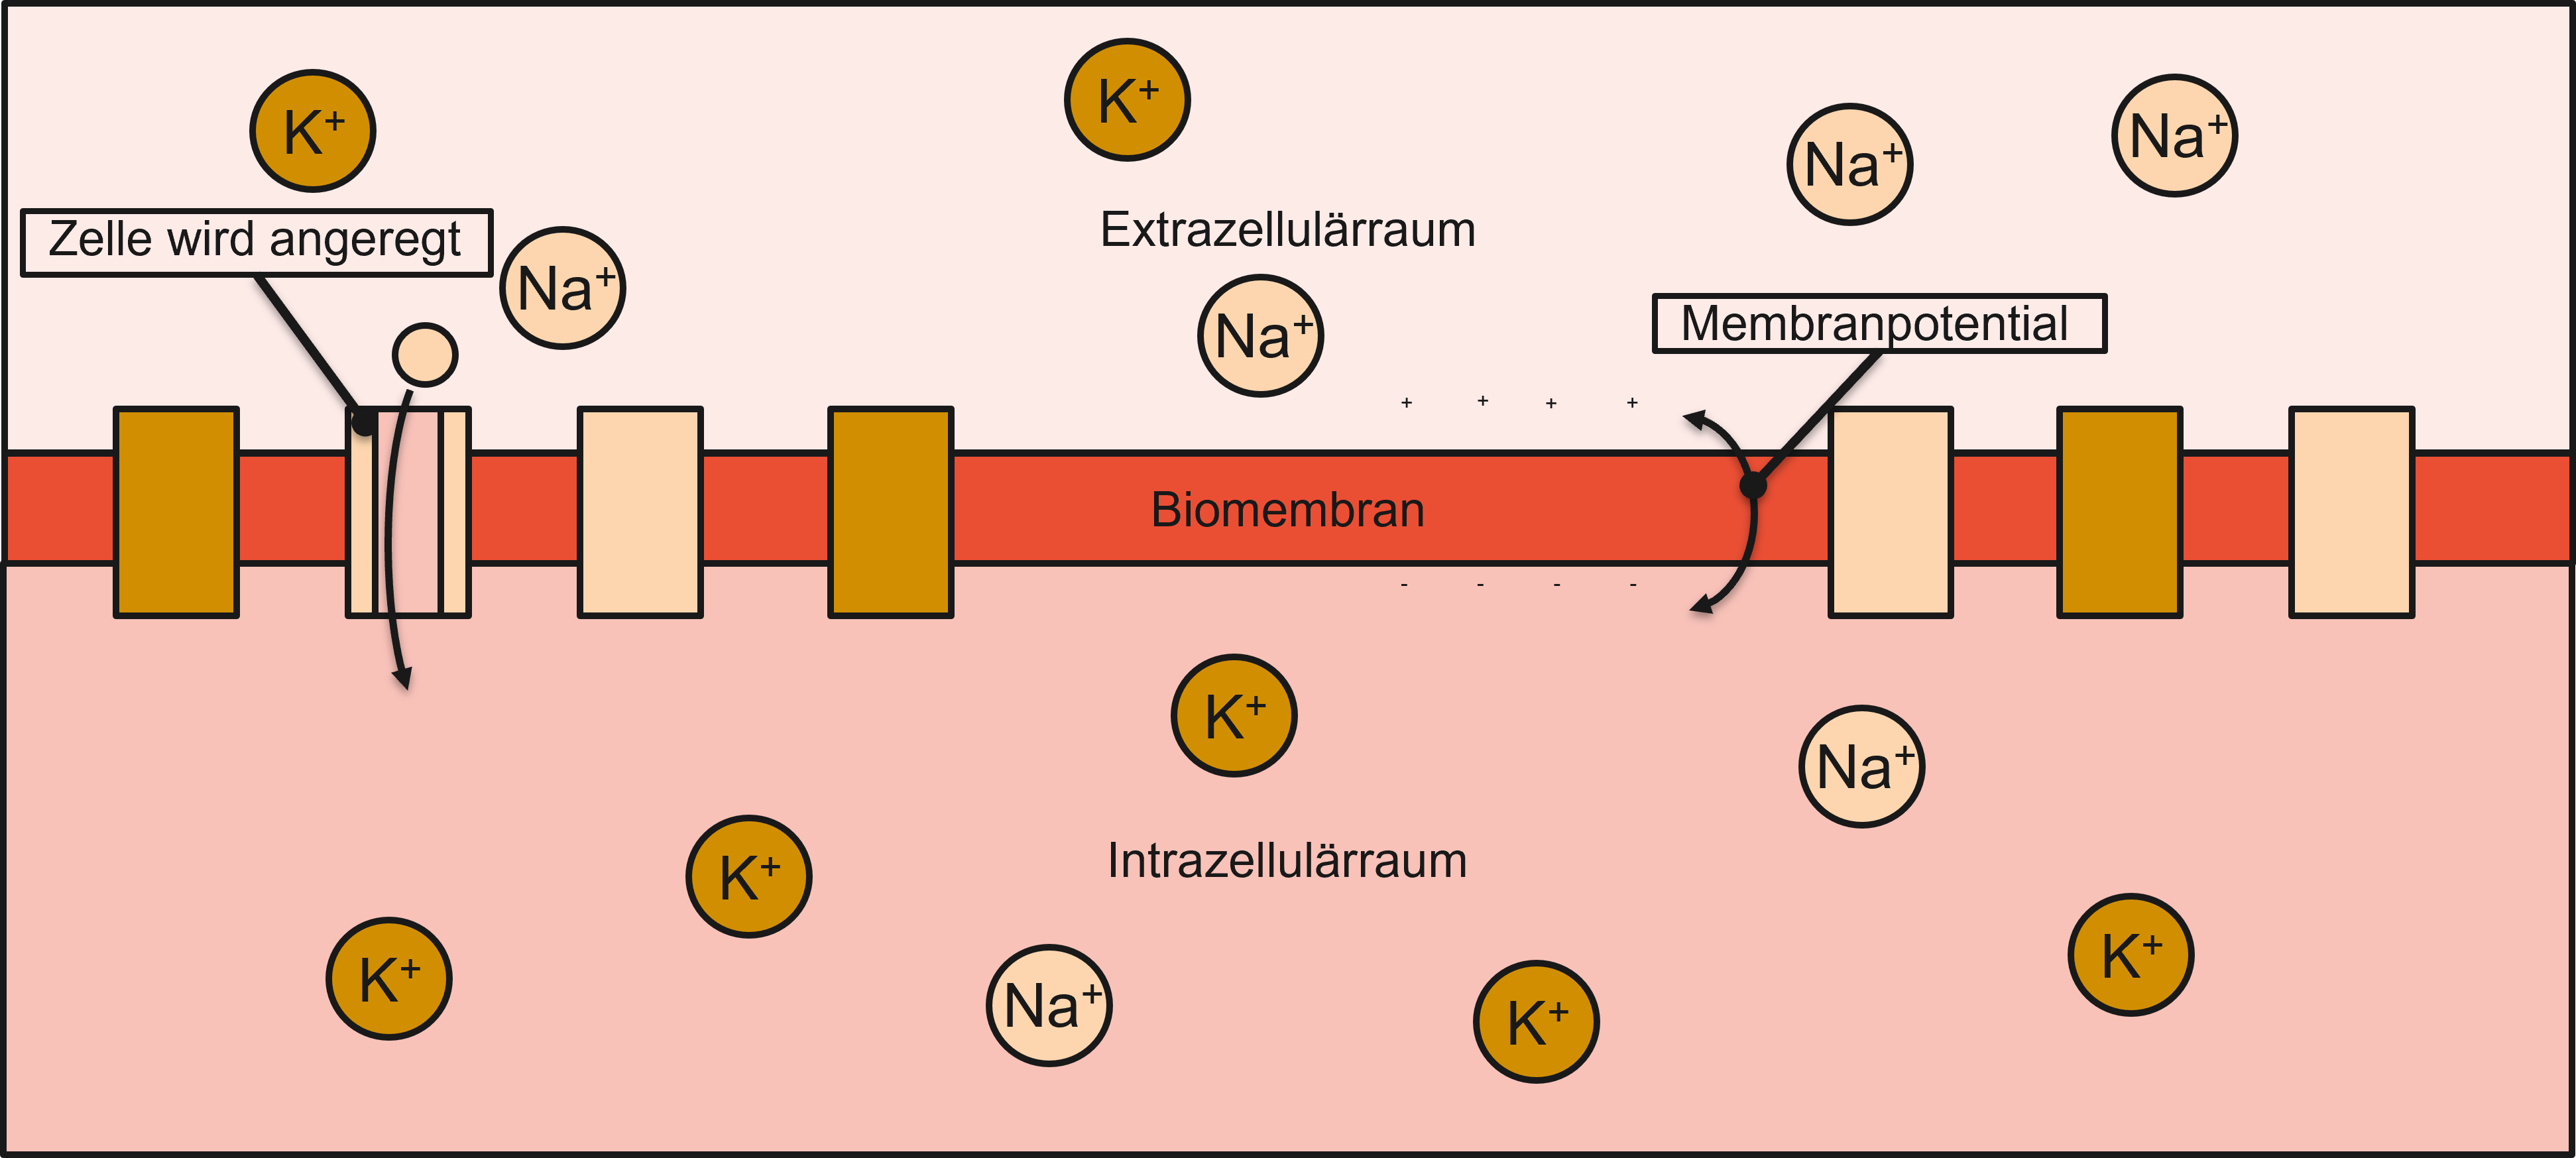
\includegraphics[width=\textwidth]{papers/nerven/Bilder/Vorgang2.png}
    \caption{Anregung: Einige Natriumionenkanalproteine öffnen sich und Natriumionen strömen in die Zelle.}
    \label{fig:Anregung}
\end{figure}

Sobald das Membranpotential grösser als der Schwellenwert von $-50$ Millivolt ist, öffnen sich wie in Abbildung
\ref{fig:Depolarisation} erkennbar schlagartig viele
Natriumkanalproteine und transportieren noch mehr Natriumionen in die Nervenzelle.
Durch diese sogenannte Depolarisation erhöht sich die Ladung der Nervenzelle noch stärker und das Membranpotential erreicht ein Maximum. 
\begin{figure}[h]
    \centering
    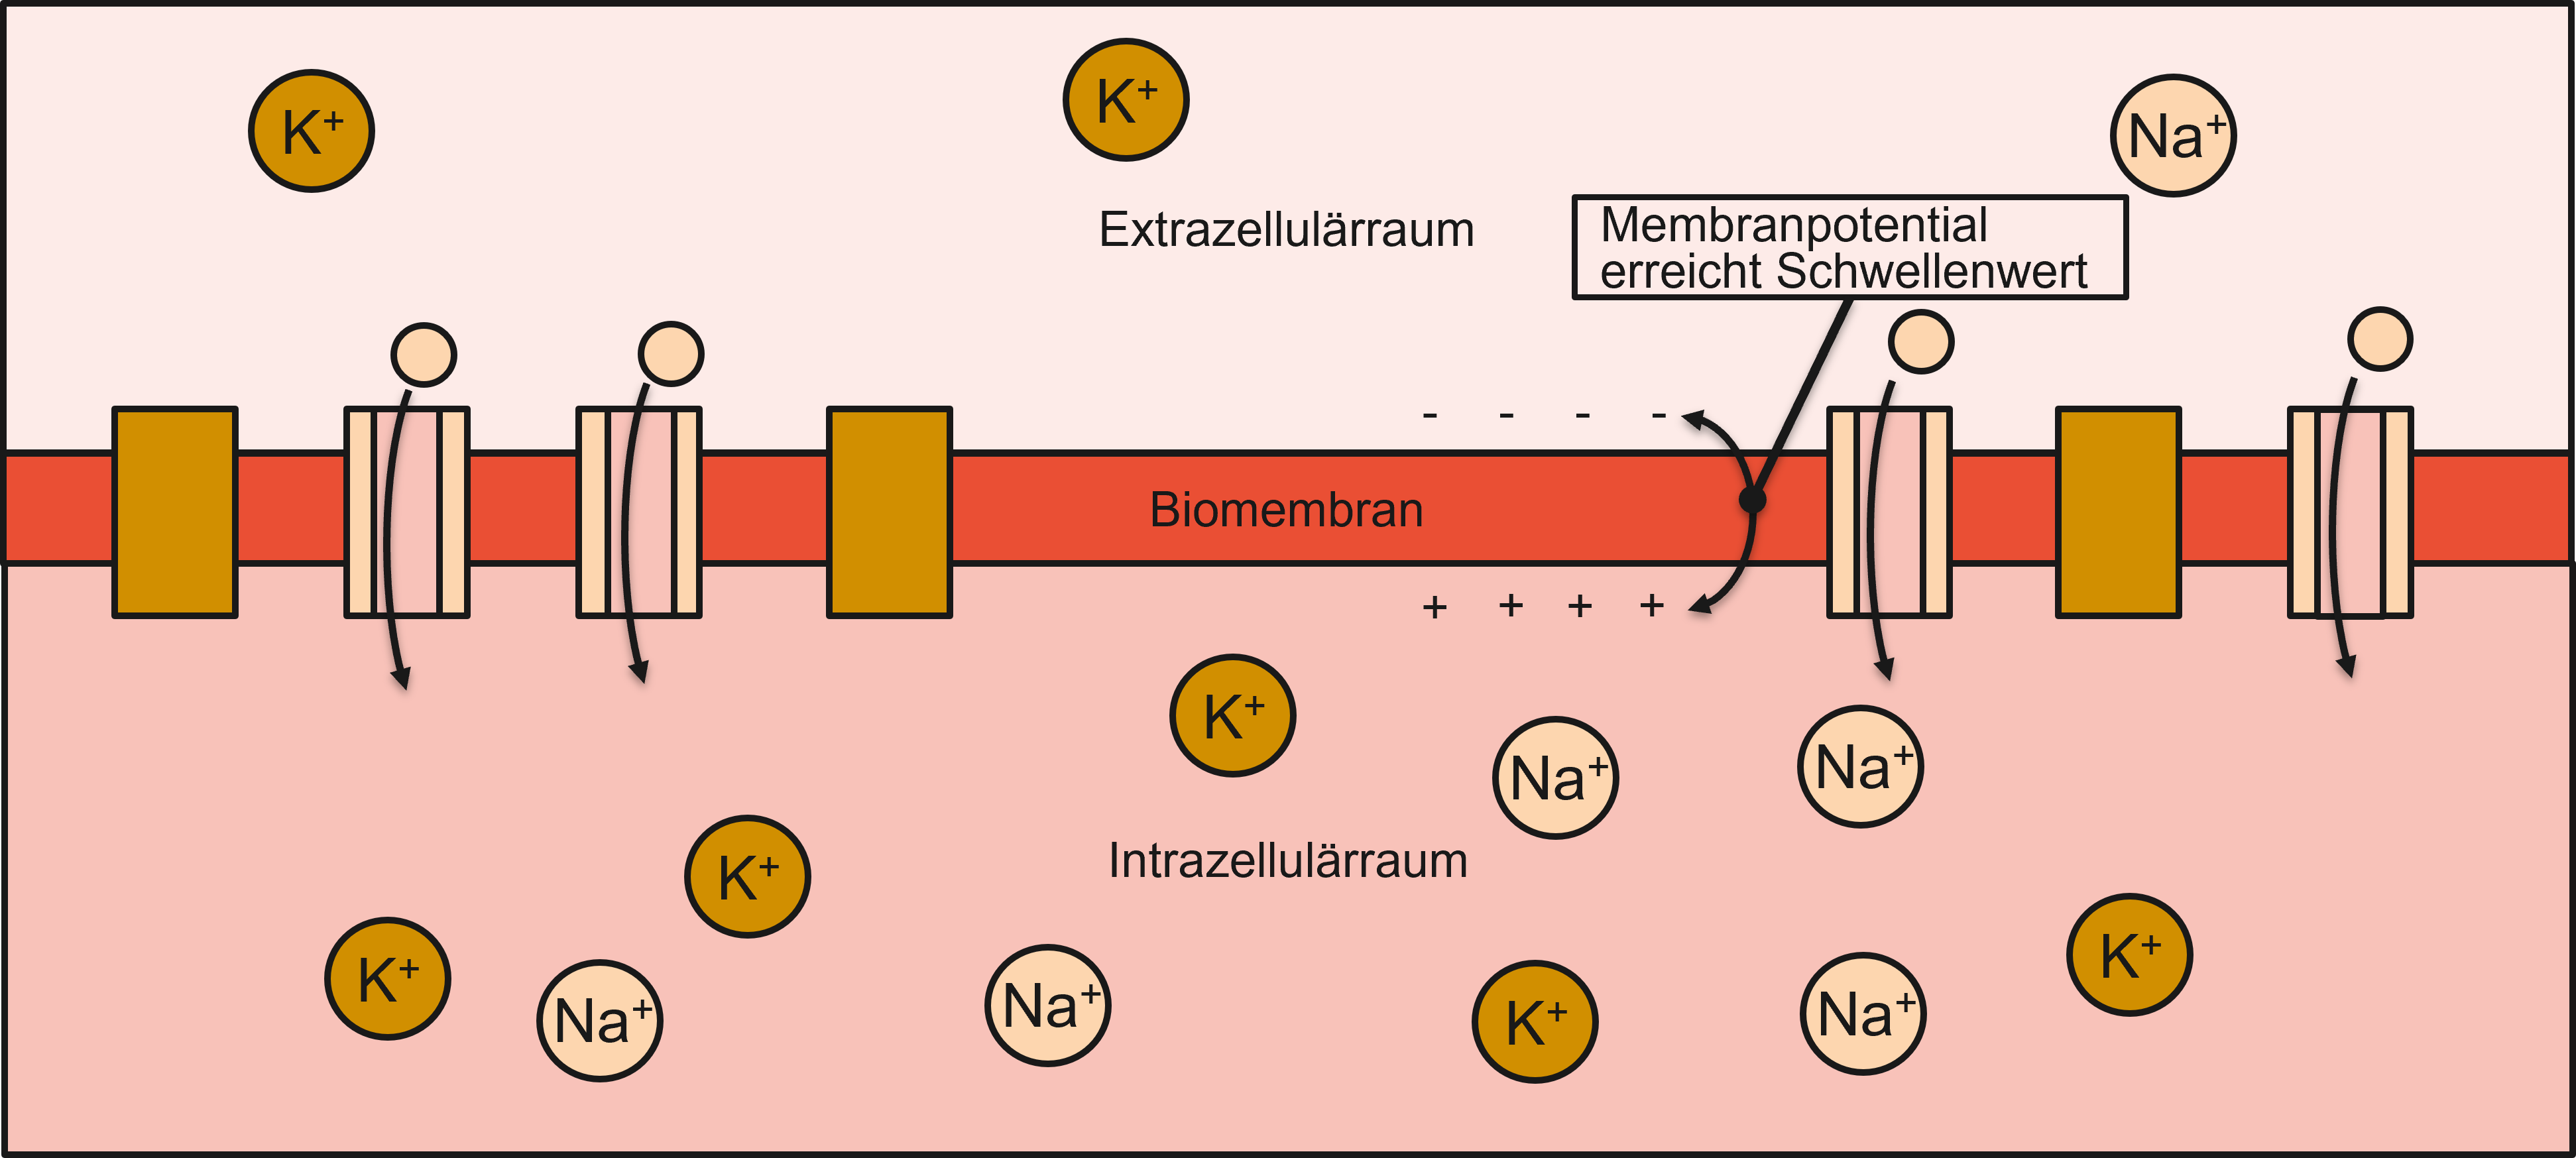
\includegraphics[width=\textwidth]{papers/nerven/Bilder/Vorgang3.png}
    \caption{Depolarisation: Beim Erreichen der Membranschwellenspannung öffnen sich alle Natriumionenkanalproteine und viele Natriumionen strömen in die Zelle.}
    \label{fig:Depolarisation}
\end{figure}

Sobald das Membranpotential sein Maximum erreicht schliessen sich die Natriumkanalproteine und dafür öffnen sich die
Kaliumkanalproteine.
Wie in Abbildung \ref{fig:Repolarisation} ersichtlich strömen viele Kaliumionen aus der Nervenzelle hinaus.
In dieser Repolarisation nimmt deshalb das Membranpotential schlagartig wieder ab.
\begin{figure}[h]
    \centering
    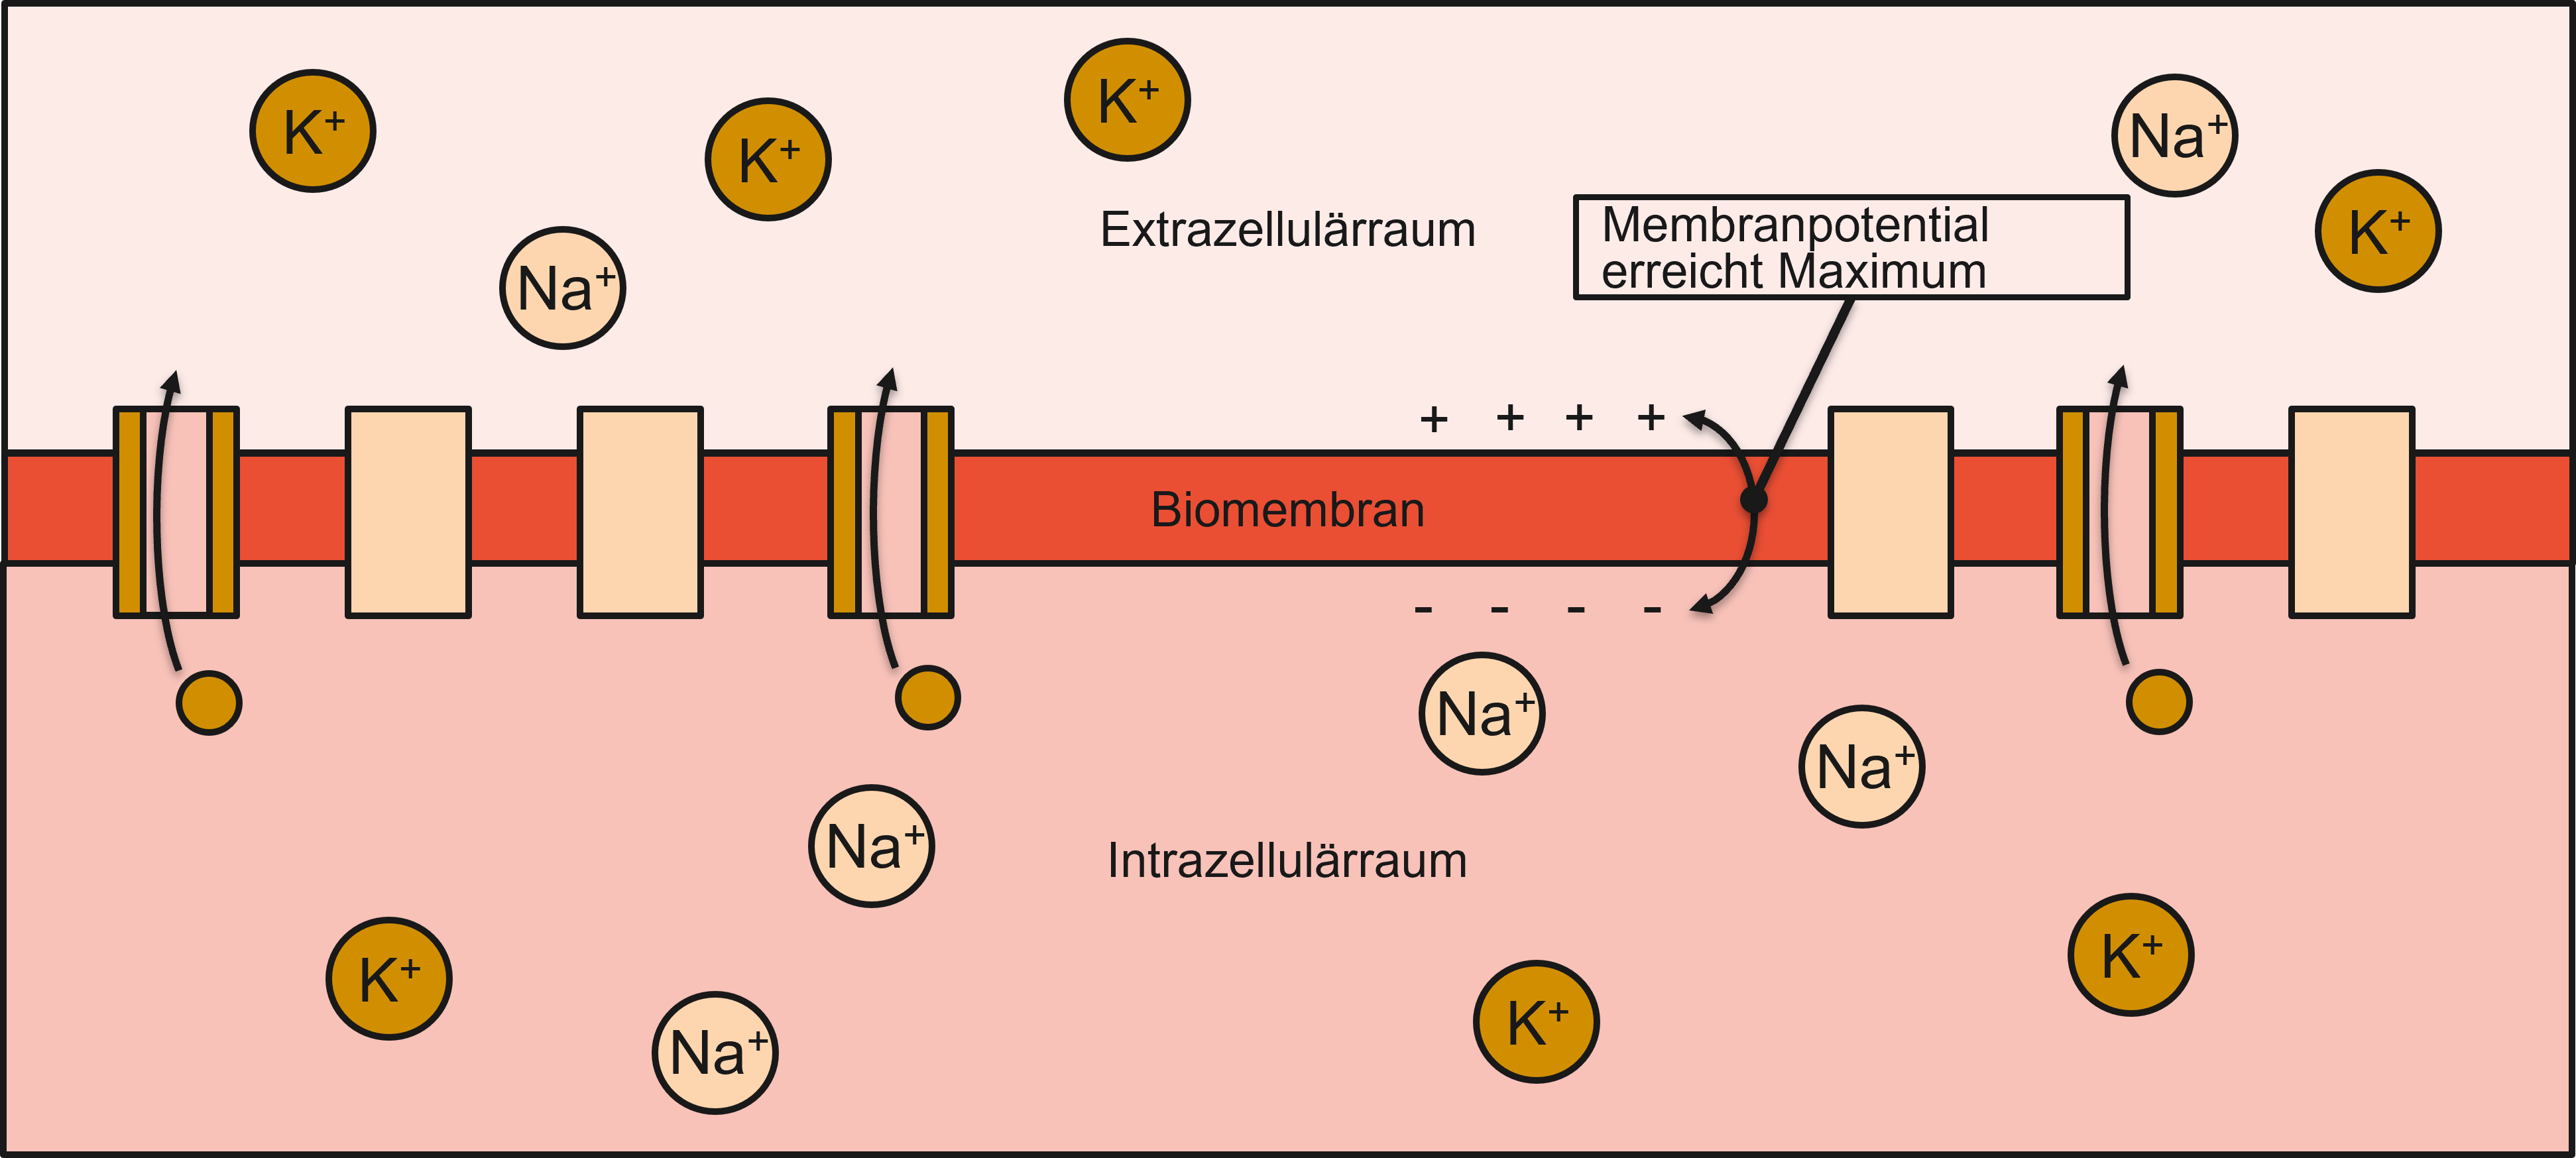
\includegraphics[width=\textwidth]{papers/nerven/Bilder/Vorgang4.png}
    \caption{Repolarisation: Beim Erreichen des Membranspannungsmaximums öffnen sich Kaliumkanalproteine und Natriumionen strömen aus der Zelle.}
    \label{fig:Repolarisation}
\end{figure}

Nachdem das Membranpotential wieder abgenommen hat, muss die Nervenzelle wieder in den Ruhezustand gelangen, dies nennt
man Hyperpolarisation.
Dafür öffnen sich, wie in Abbildung \ref{fig:Hyperpolarisation} ersichtlicht, Kanalproteine für beide Ionen und durch die
Ionenpumpe strömen Kaliumionen in die Zelle und Natriumionen aus der Zelle.
Durch die ungleiche Verteilung von Natrium- und Kaliumionen ensteht so wieder ein negatives Membranpotential an der Zellenwand.
\begin{figure}[h]
    \centering
    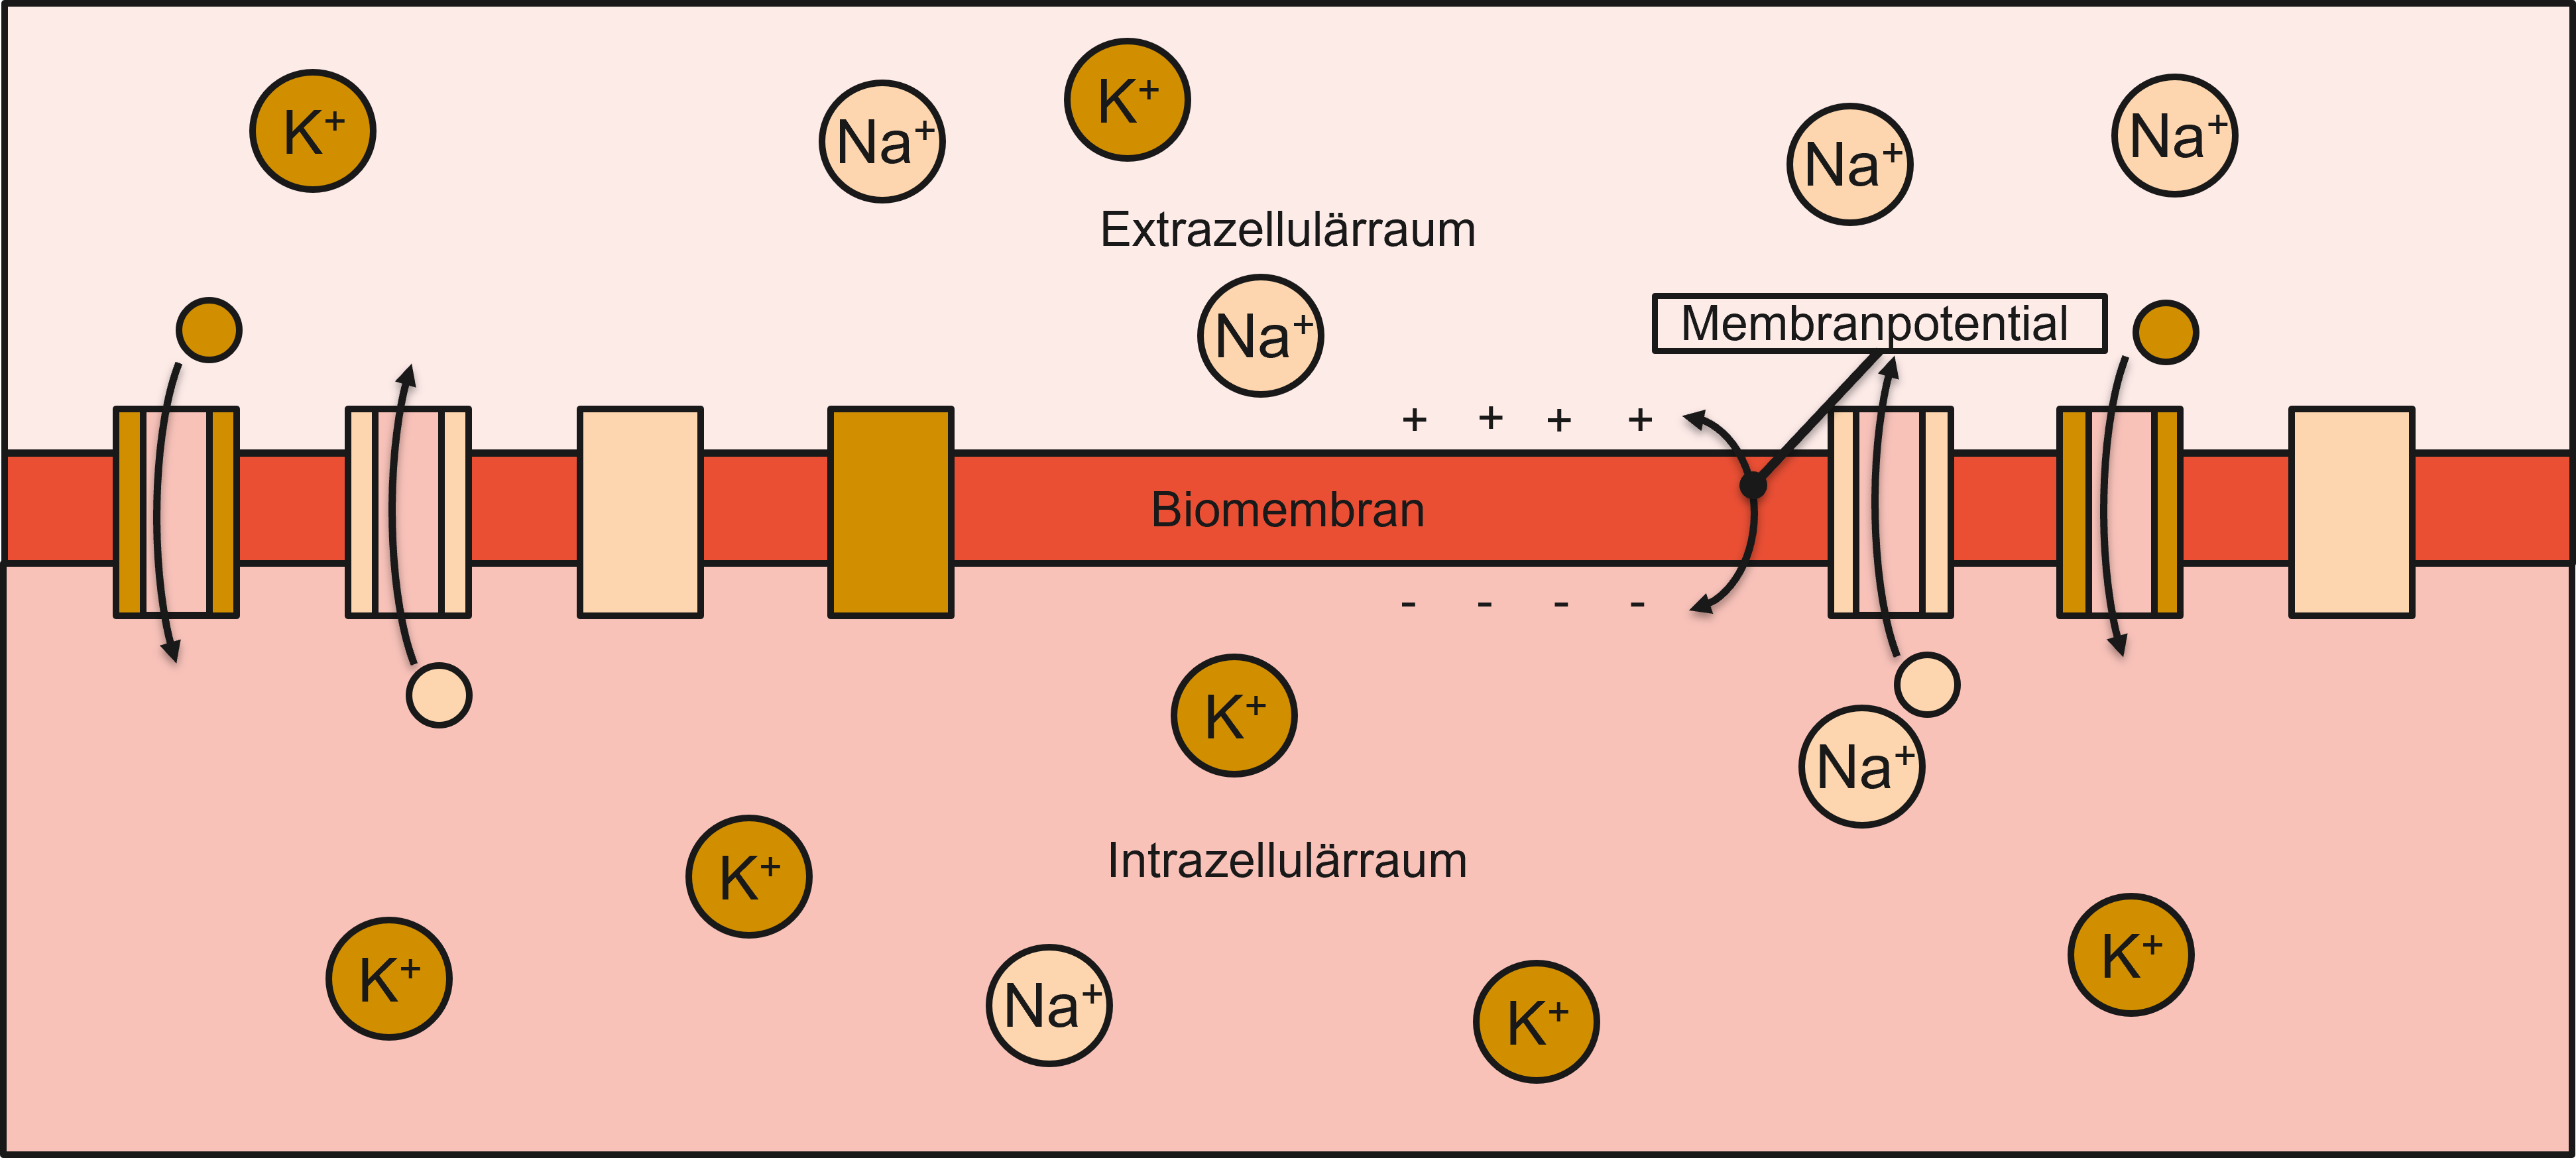
\includegraphics[width=\textwidth]{papers/nerven/Bilder/Vorgang5.png}
    \caption{Hyperpolarisation: Die Nervenzelle gleicht die Ionenkonzentration wieder aus um den Ruhezustand zu erreichen.}
    \label{fig:Hyperpolarisation}
\end{figure}
\section{Hodgkin-Huxley Modell}
\subsection{Einleitung}
Das Hodgkin-Huxley-Modell wurde 1952 von den britischen Physiologen Alan Hodgkin und Andrew Huxley entwickelt. Es beschreibt das elektrophysiologische Verhalten von Nervenzellen, genauer gesagt den Aktionspotentialverlauf entlang einer Nervenfaser. Das Modell basiert auf experimentellen Messungen am Riesenaxon des Tintenfisches und erklärt, wie sich die elektrische Spannung entlang einer Nervenzelle über die Zeit verändert. Dieses Modell wurde zum ersten Mal erfolgreich verwendet, um den komplexen Ionenfluss durch die Zellmembran quantitativ zu beschreiben. Es bildet die Grundlage für viele spätere Modelle wie das FitzHugh-Nagumo-Modell, welches in dieser Arbeit vertiefter behandelt wird 
\cite{nerven:InaLammers.31.08.2015}.
\subsection{Nutzen}
Der grösste Beitrag des Hodgkin-Huxley-Modells liegt in der mathematischen Beschreibung der biologischen Realität: Es verbindet biologische Prozesse wie Natrium- und Kaliumkanalbewegungen mit einem nichtlinearer Differentialgleichungenssystem. Das Modell erklärt das Zustandekommen eines Aktionspotentials und erlaubt Simulationen und Vorhersagen für Nervenreaktionen auf Reize. Es ist bis heute in der Neuroinformatik, Biophysik und mathematischen Neurowissenschaft von zentraler Bedeutung und diente als Grundlage für realistische neuronale Netzwerke 
\cite{nerven:InaLammers.31.08.2015}.
\subsection{Mathematische Grundlage}
Das Hodgkin-Huxley-Modell basiert auf der elektrischen Leitfähigkeit der Membrane und stellt die Nervenmembran als ein elektrisches Schaltbild dar, welches eine Kapazität $C_m$ sowie mehrere stromleitende Kanäle für spezifische Ionen umfasst.
Die fundamentale Gleichung ist der einzige Ausschnitt des Hodgkin-Huxley-Model welche aus natürlichen und biologischen Beobachtungen entstanden ist, die restlichen Gleichungen und Beobachtungen hängen nicht deutlich von molekularen Mechanismen zusammen. 
Das Membranpotential $V$ erfüllt beim Hodgkin-Huxley-Modell die Differentialgleichung: 
\[C_m \frac{dV}{dt} = I_{\text{ext}} - (I_{\text{Na}} + I_{\text{K}} + I_L)\] 
\noindent
Dabei ist:

\begin{itemize}
	\item $V(t)$: Membranpotential (mV)
	\item $C_m$: Membrankapazität pro Fläche ($\mu$F/cm$^2$)
	\item $I_{\text{ext}}$: externer Reizstrom
	\item $I_{\text{Na}}, I_{\text{K}}$: Natrium- und Kaliumströme
	\item $I_L$: Leckstrom
\end{itemize}
\subsubsection{Ionenströme}
Die Ionenströme sind spannungs- und zeitabhängig. Sie folgen jeweils einer eigenen Formel, nämlich:
\[
\begin{aligned}
	I_{\text{Na}} &= \bar{g}_{\text{Na}} \cdot m^3 h \cdot (V - E_{\text{Na}}), \\
	I_{\text{K}} &= \bar{g}_{\text{K}} \cdot n^4 \cdot (V - E_{\text{K}}), \\
	I_L &= \bar{g}_L \cdot (V - E_L).
\end{aligned}
\]
\noindent
Dabei ist:

\begin{itemize}
	\item $\bar{g}_{\text{Na}},\, \bar{g}_{\text{K}},\, \bar{g}_L$: maximale Leitfähigkeiten (Konstanten)
	\item $E_{\text{Na}}, E_{\text{K}}, E_L$: Umkehrpotentiale der Ionen
	\item $m, h, n$: \emph{Torvariablen}, die zwischen 0 und 1 schwanken und die Öffnungswahrscheinlichkeit von Ionenkanälen angeben
\end{itemize}
Die Torvariablen $m$, $h$ und $n$ sind Variablen, die keine reine biologische Überlegungen haben, sondern durch vielen Testversuchen entstanden sind. Diese Torvariablen werden so angepasst, dass die Dynamik bei den Natrium- und Kaliumionenkanälen erklärt wird.
\subsubsection{Dynamik der Torvariablen}
Die Torvariablen folgen jeweils Differentialgleichungen erster Ordnung, z. B.:

\begin{align}
	\frac{dn}{dt} &= \alpha_n (1 - n) - \beta_n n \\
	\frac{dm}{dt} &= \alpha_m (1 - m) - \beta_m m \\
	\frac{dh}{dt} &= \alpha_h (1 - h) - \beta_h h 
\end{align}

Dabei sind $\alpha_m$ und $\beta_m$ spannungsgesteuerte Übergangsraten, die empirisch durch Hodgkin und Huxley bestimmt wurden.
Diese Differentialgleichungen beschreiben wie $m$, $h$ und $n$ jeweils vom Membranpotential $V$ abhängig sind.
\subsubsection{Mathematische Einordnung der Gleichung}
Mathematisch handelt es sich beim Hodgkin-Huxley-Modell um ein System von vier gekoppelten nichtlinearen
Differentialgleichungen:
\begin{itemize}
    \item Eine Gleichung für das Membranpotential $V(t)$
    \item Drei Gleichungen für die Torvariablen $m(t)$, $h(t)$, $n(t)$
\end{itemize}
Es gehört zur Klasse der nichtlinearen dynamischen Systeme, genauer gesagt zu einem System von gewöhnlichen Differentialgleichungen. Die Nichtlinearität entsteht durch die Potenzen (z. B. $m^3$) und das Produkt der Torvariablen mit $V$.
\subsubsection{Fazit}
Das Hodgkin-Huxley-Modell ist nicht nur ein Meilenstein der Biologie, sondern auch ein Paradebeispiel dafür, wie mathematische Modellierung biologische Prozesse quantitativ erfassen kann. Die Gleichungen geben Verständnis über die Entstehung und Ausbreitung elektrischer Signale in Nervenzellen und sind bis heute unverzichtbar in der Neurophysik und mathematischen Biologie.

\section{FitzHugh-Nagumo-Modell}
Das FitzHugh-Nagumo-Modell ist eine mathematische Vereinfachung des Hodgkin-Huxley-Modells. Entwickelt wurde es in den 1960er-Jahren von Richard FitzHugh und Jinichi Nagumo, um die komplexe Dynamik des neuronalen Aktionspotentials auf ein qualitativ ähnliches, aber mathematisch reduziertes System zurückzuführen.
Das Modell vereinfacht die Nervenaktivität auf zwei Hauptvariablen, eines ist das Membranpotential $v(t)$ und eines die Erholungsvariable $w(t)$, die langsame Rückstellprozesse modelliert.
Ziel war es, ein System zu formulieren, das zwar die fundamentalen Eigenschaften wie Reizantwort, Erregbarkeit und Rückkehr zum Ruhezustand bewahrt, aber deutlich einfacher zu analysieren ist 
\cite{nerven:InaLammers.31.08.2015}.
\subsubsection{Nutzen des FitzHugh-Nagumo-Modells}
Das FitzHugh-Nagumo-Modell erlaubt eine qualitative Analyse neuronaler Aktivität mit einfachen Mitteln:
\begin{itemize}
    \item Simulation von Aktionspotentialen
    \item Beschreibung von Refraktärzeiten
    \item Untersuchung der Stabilität von Ruhezuständen
    \item Analyse von Schwellwertverhalten bei Reizen
    \item Einsatz in räumlich ausgedehnten Modellen (z.B. als Reaktions-Diffusions-System für Ausbreitung von Signalen im Gewebe)
\end{itemize}

Gerade in der Mathematik ist das Modell besonders beliebt, da es sich ideal für phasenraumanalytische Methoden eignet,
insbesondere für die Betrachtung von Nullklinen, Fixpunkten und Grenzzyklen 
\cite{nerven:InaLammers.31.08.2015}.
\subsubsection{Mathematische Beschreibung des Modells}
Das FitzHugh-Nagumo-Modell besteht aus einem System zweier gekoppelter nichtlinearer Differentialgleichungen erster Ordnung:
Diese Differentialgleichung wurden aus der fundamentalen Formel des Hodkin-Huxley-Modell hergeleitet, jedoch ist diese Herleitung sehr komplex und wird in dieser Arbeit nicht weiter erklärt. Aus der fundamentalen Formel vom Hodkin-Huxley-Modells werden die folgenden gekoppelten nichtlinearen Differentialgleichung erster Ordnung:
\[
\begin{aligned}
	\frac{dv}{dt} &= v - \frac{v^3}{3} - w + I_{\text{ext}} \\
	\frac{dw}{dt} &= \varepsilon (v + a - b w).
\end{aligned}
\]
\noindent
Dabei ist:

\begin{itemize}
	\item $v(t)$: Membranpotential (schnelle Variable)
	\item $w(t)$: Erholungsvariable (langsame Variable)
	\item $I_{\text{ext}}(t)$: externer Reizstrom
	\item $\varepsilon \ll 1$: kleine Konstante, die die Zeitskalen trennt (Langsamkeit von $w$)
	\item $a, b$: Systemparameter, die die Dynamik und Stabilität beeinflussen
\end{itemize}
Das ist ein zweidimensionales, also ebenes System von gewöhnlichen Differentialgleichungen. Dies veringert den mathematischen Aufwand und macht es uns sehr einfach, Eigenschaften mithilfe des Modells zu indentifizieren.
Mit $w$ und $v$ als stetig und differenzierbaren Funktion sind die Ergebnisse mithilfe von Nullklinien (welche in den nächsten Unterkapiteln erklärt werden) sehr leicht zu finden.

Interpretation:
\begin{itemize}
    \item Die erste Gleichung beschreibt die schnelle Aktivierung des Neurons: sie enthält eine nichtlineare Rückkopplung durch den Term $v^3$, die für die typische „Spike“-Form des Aktionspotentials sorgt.
    \item Die zweite Gleichung reguliert die langsame Erholung und Rückführung zum Ruhezustand.
\end{itemize}
\subsubsection{Mathematische Einordnung}
Das FitzHugh-Nagumo-Modell ist ein typisches Beispiel für ein Relaxationsoszillator-system, bei dem zwei Variablen auf unterschiedlichen Zeitskalen miteinander gekoppelt sind. Solche Systeme sind bekannt für:
\begin{itemize}
	\item Sprunghaftes Verhalten (z. B. plötzlicher Aktionspotentialanstieg)
	\item Rückkehr zum Ausgangszustand (Refraktärphase)
	\item Nichtlineare Dynamik mit Sättigung und Schwellenwertverhalten
\end{itemize}
Mathematisch ist es ein nichtlineares System von gewöhnlichen Differentialgleichungen.
\subsubsection{Analyse der Nullklinen}
Die Nullklinen sind die geometrischen Orte im Phasenraum ($v$,$w$), an denen die jeweilige Zeitableitung einer Variable verschwindet (d. h. gleich null ist). Sie stellen somit die Punkte dar, in denen sich die entsprechende Variable nicht mehr ändert, und sind ein zentrales Werkzeug zur Analyse des Systems. Sie sind ein zentrales Werkzeug zur Analyse des Systems.

\emph{v-Nullkline:} $\dfrac{dv}{dt} = 0$
\noindent
 ,Setze:
\[
v - \frac{v^3}{3} - w + I_{\text{ext}} = 0
\]

\noindent
Nach $w$ umgestellt:
\[
w = v - \frac{v^3}{3} + I_{\text{ext}}
\]

Das ist eine \emph{kubische Kurve} im Phasenraum, typischerweise mit \emph{S-Form}.  
Sie gibt an, wo das Membranpotential im Gleichgewicht ist (für festes $w$).

\vspace{1em}

\emph{w-Nullkline:} $\dfrac{dw}{dt} = 0$
\noindent
Setze:
\[
\varepsilon (v + a - b w) = 0 \Rightarrow v + a - b w = 0 \Rightarrow w = \frac{v + a}{b}.
\]
Das ist eine Gerade im Phasenraum.  
Sie gibt an, wo sich die Erholungsvariable im Gleichgewicht befindet (für festes $v$).
Der Schnittpunkt beider Nullklinen ist ein Gleichgewichtspunkt des Systems: Dort gilt sowohl $\frac{dv}{dt} = 0$ als
auch $\frac{dw}{dt} = 0$. Dieser Punkt kann je nach Parametern stabil oder instabil sein.
\subsubsection{Bedeutung}
Das Verhalten des Systems kann durch die Phasenporträtanalyse qualitativ vorhergesagt werden:
\begin{itemize}
	\item Wenn der Fixpunkt stabil ist, kehrt das System nach einem kleinen Reiz dorthin zurück → Ruhe.
	\item Bei instabilem Fixpunkt (Sattel, Fokus) kommt es zu Grenzzyklen → rhythmisches Feuern.
	\item Der Verlauf der Trajektorien im Phasenraum zeigt den zeitlichen Verlauf des Aktionspotentials.
\end{itemize}
Die S-Form der $v$-Nullkline erzeugt Sprungdynamik:
\begin{itemize}
	\item Linker Ast: Ruhe
	\item Mittlerer Ast: instabil (Schwellwert)
	\item Rechter Ast: Aktivierung („Spike“)
\end{itemize}
Das FitzHugh-Nagumo-Modell ist eine elegante und reduktive Darstellung neuronaler Erregung, das die komplexe Biologie auf zwei mathematisch gut fassbare Prozesse reduziert. Seine Stärke liegt in der Analyse der Dynamik im Phasenraum, insbesondere über die Nullklinen und Fixpunkte. Es eignet sich hervorragend zur Simulation, Theoriebildung, Lehre und bildet eine solide mathematische Brücke zwischen Biologie und dynamischer Systemtheorie.

\section{Verhalten bei Anregung}
\subsection{Formelparameter}
In den vorigen Abschnitten wurden die Parameter der Nullklinien des Fitzhugh-Nagumo Modells folgendermassen definiert:
\(a = -0.7, b = 0.8, \epsilon = 0.8, I_\text{ext} = 0\). Somit werden aus den allgemeinen Nullklinien \[ w = v - \frac{v^3}{3} + I_{ext}\]
und \[w = \frac{v + a}{b}\] die spezifischen Nullklinien \[ w = v - \frac{v^3}{3}\]
und \[w = \frac{v + 0.7}{0.8}.\]
Der stationäre Punkt, welcher von Objekten im Vektorfeld angestrebt werden, befindet sich bei $(1.2 ,-0.6)$.
Der Parameter $I_\text{ext}$ ist als 0 definiert, dies bedeutet, es findet keine Anregung statt.
In Abbildung \ref{fig:Parameter} sind das Vektorfeld und die Nullklinien erkennbar, wenn das Modell nicht angeregt wird.
\begin{figure}[h]
    \centering
    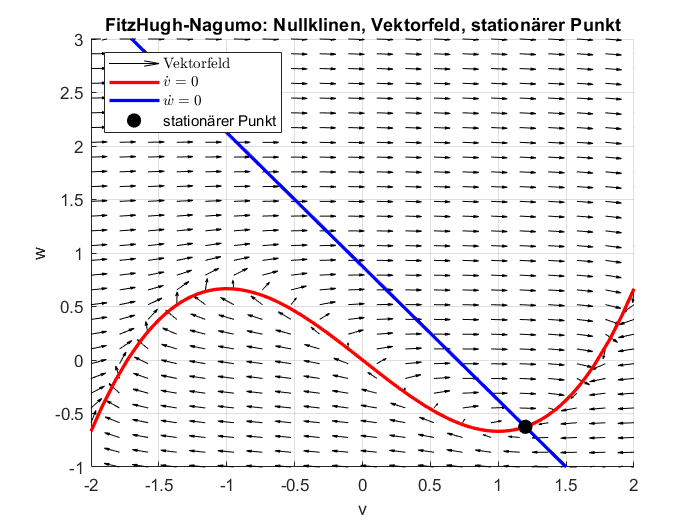
\includegraphics[width=0.9\textwidth]{papers/nerven/Bilder/Anregung1.png}
    \caption{Vektorfeld, Nullklinien und stationärer Punkt}
    \label{fig:Parameter}
\end{figure}
\subsection{Schwache Anregung}
Wenn das Fitzhugh-Nagumo-Modell angeregt werden soll, muss der Parameter $I_\text{ext}$ verändert werden.
Beispielweise kann $I_\text{ext} = 0.1$ Volt definiert werden.
Dadurch wird die $v$-Nullklinie um 0.1 in positive $w$-Richtung verschoben.
Somit verändern sich die Nullklinien zu \[ w = v - \frac{v^3}{3} + 0.1\]
und \[w = \frac{v + 0.7}{0.8}\] und der stationäre Punkt wandert zu $(1.1 ,-0.5)$.
Der ursprüngliche stationäre Punkt ist jetzt nicht mehr stabil und wird vom Vektorfeld in den neuen stationären Punkt
gezwungen.
Dies geschieht entlang des Vektorfelds, was bei dieser schwachen Anregung nur eine kurze Trajektorie ergibt.
In Abbildung \ref{fig:schwacheAnregung} lässt sich die Trajektorie zwischen den stationären Punkten erkennen, sowie
deren Auslenkung in $v$-Richtung.
Da die Anregung von $I_\text{ext} = 0.1$ sehr schwach ist, fällt auch die Auslenkung der Trajektorie in $v$-Richtung mit 0.2 klein aus und
nimmt sofort wieder ab. 
Dieser Effekt tritt auf, wenn die Nervenzelle mit einer Spannung unterhalb der Schwellenspannung angeregt wird.
\begin{figure}[h]
    \centering
    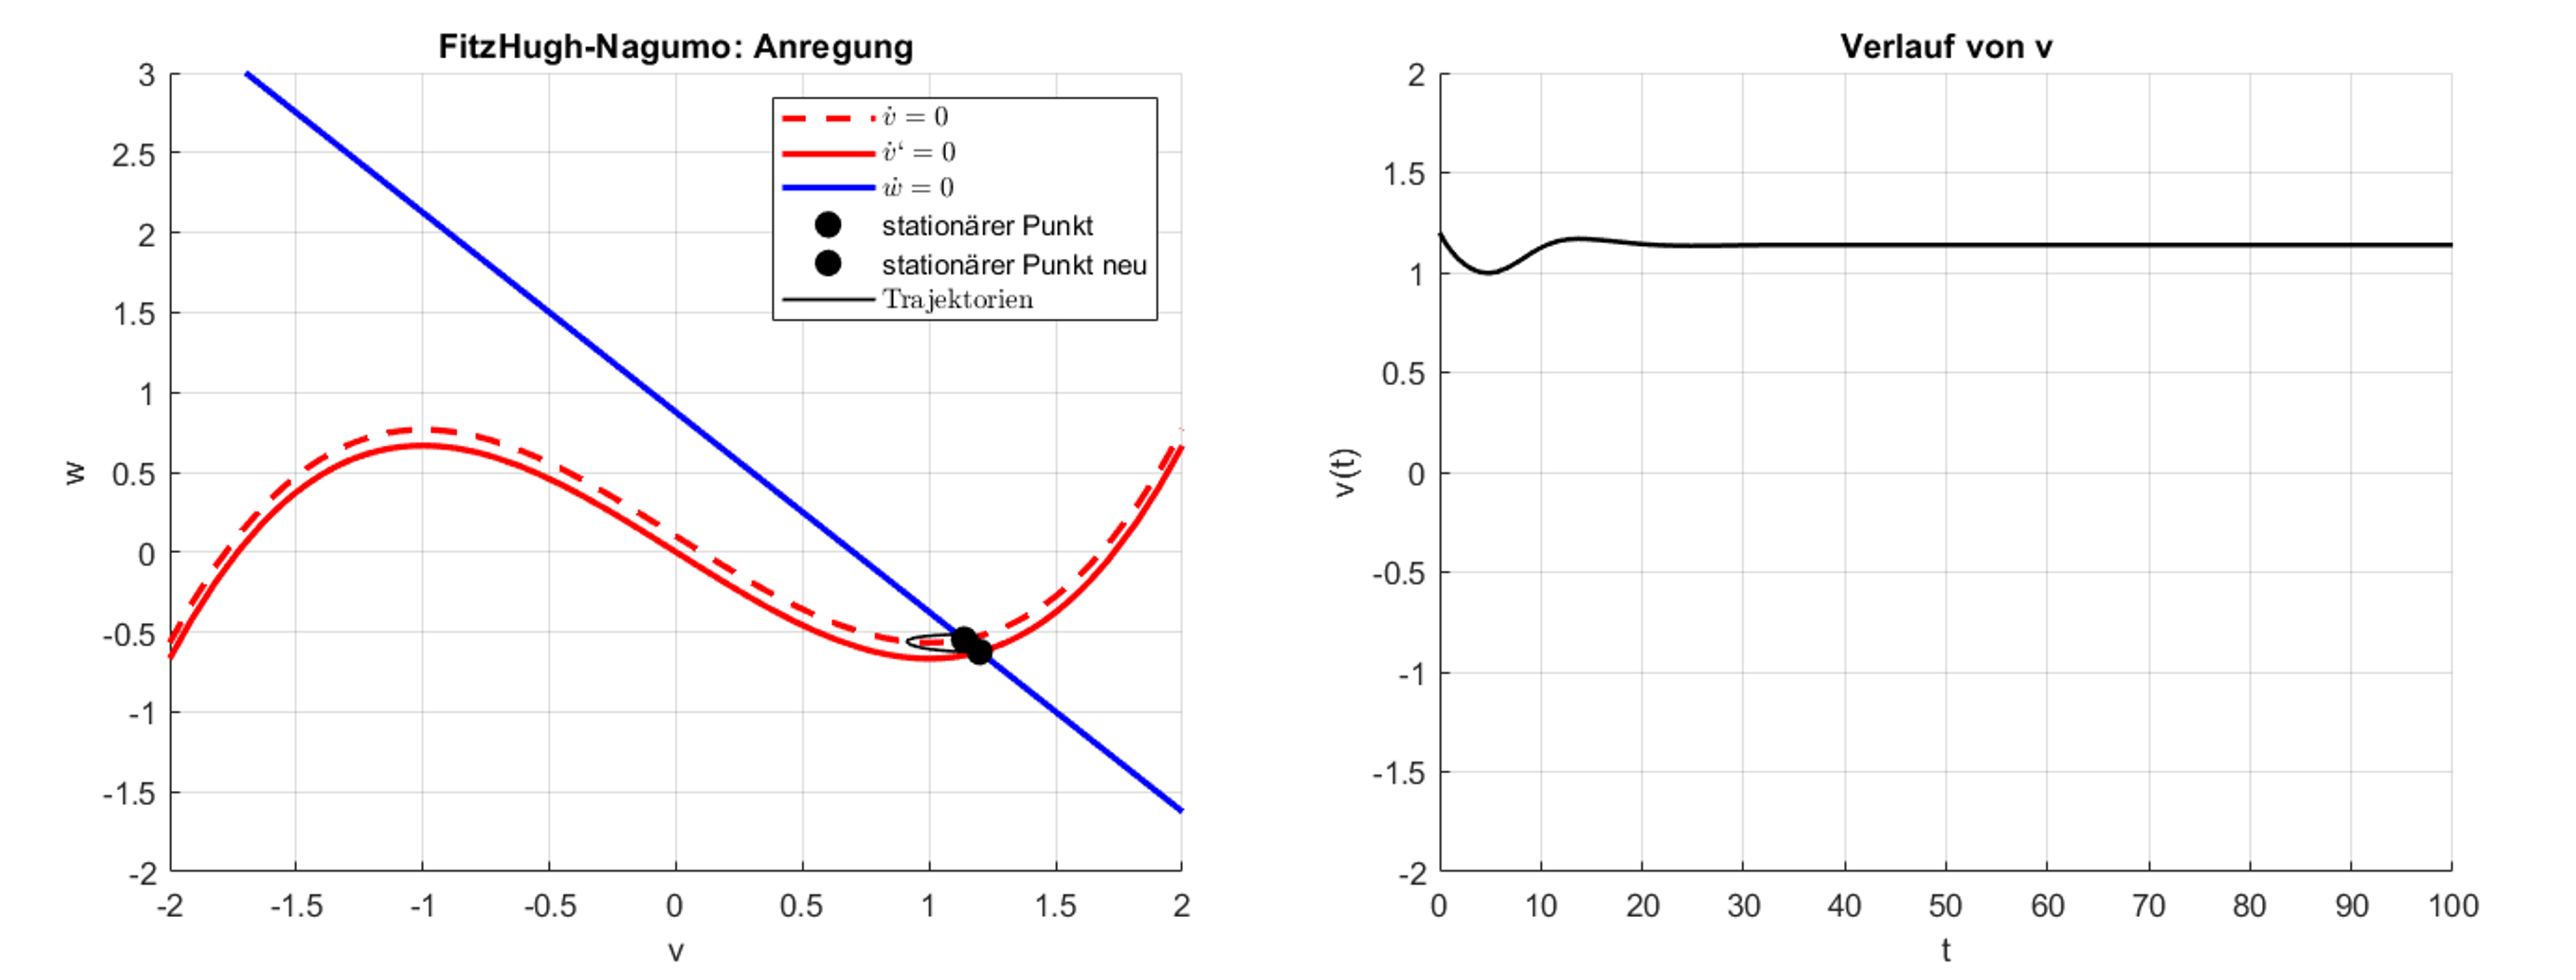
\includegraphics[width=\textwidth]{papers/nerven/Bilder/schwacheAnregung.png}
    \caption{Schwache Anregung des Fitzhugh-Nagumo-Modells}
    \label{fig:schwacheAnregung}
\end{figure}
\subsection{Starke Anregung}
Um den Effekt, der bei einer Nervenzelle bei Anregung über der Schwellenspannung auftritt, beobachten zu können, muss
der Parameter $I_\text{ext}$ erhöht werden.
Beispielweise wird hier $I_\text{ext} = 0.3$ Volt definiert.
Dadurch wird die $v$-Nullklinie um 0.3 in positive w-Richtung verschoben.
Somit verändern sich die Nullklinien zu 
\[ w = v - \frac{v^3}{3} + 0.3\]
und \[w = \frac{v + 0.7}{0.8}\] und der stationäre Punkt wandert zu $(1 ,-0.3)$.
Der ursprüngliche stationäre Punkt wird wieder instabil und vom Vektorfeld in den neuen stationären Punkt
gezwungen.
Dies geschieht entlang des Vektorfelds, was bei dieser stärkeren Anregung eine lange Trajektorie ergibt.
In Abbildung \ref{fig:starkeAnregung} lässt sich die Trajektorie zwischen den stationären Punkten erkennen, sowie
deren Auslenkung in $v$-Richtung.
Durch das Vektorfeld muss der ursprüngliche stationäre Punkt, bei einer Anregung von $I_\text{ext} = 0.3$ eine grosse Kurve
beschreiben um den neuen stationären Punkt zu erreichen.
Die Auslenkung in $v$-Richtung ist dadurch mit $-3$ auch viel grösser und es lässt sich ein impulsartiger Verlauf erkennen.
\begin{figure}[H]
    \centering
    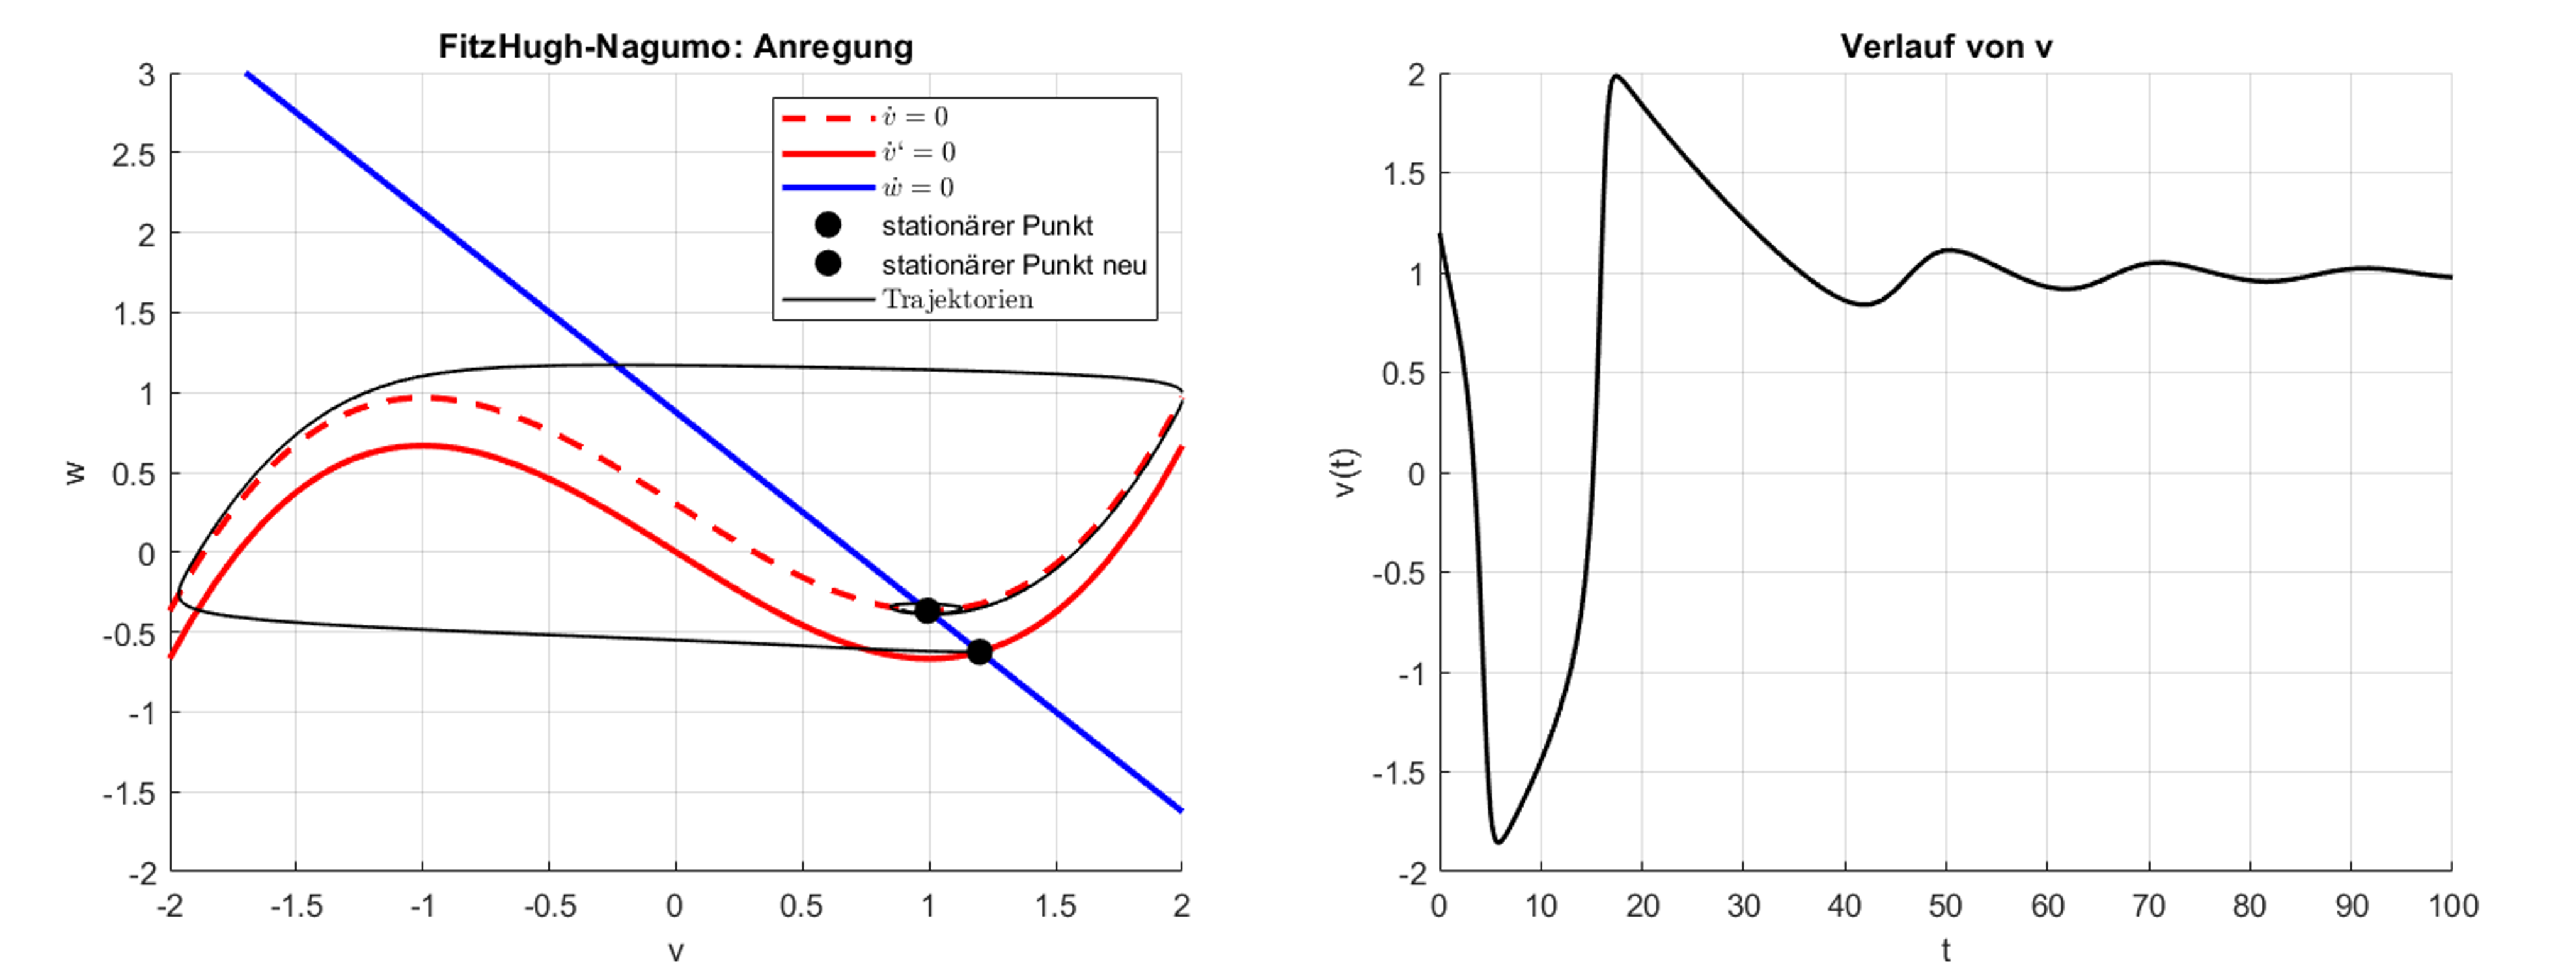
\includegraphics[width=\textwidth]{papers/nerven/Bilder/starkeAnregung.png}
    \caption{Starke Anregung des Fitzhugh-Nagumo-Modells}
    \label{fig:starkeAnregung}
\end{figure}
\subsection{Vergleich mit Aktionspotential}
Der Verlauf der Auslenkung der Trajektorie in $v$-Richtung bei einer starken Anregung des FitzHugh-Nagumo-Modell, lässt
sich mit dem Verlauf des Aktionspotentials der Nervenzelle vergleichen. 
In Abbildung \ref{fig:Vergleich} sind links die Auslenkung in $v$-Richtung und rechts der Verlauf des Aktionspotentials
erkennbar.
Der Verlauf der Auslenkung in $v$-Richtung ist an der $v$-Achse gespiegelt, um die Abbildungen besser vergleichen zu können.
In der Abbildung lassen sich die einzelnen Phasen: Depolarisation, Repolarisation und Hyperpolarisation erkennen, die
sowohl im Verlauf der Auslenkung in $v$-Richtung und im Verlauf des Aktionspotentials auftreten.
Somit kann mit dem Nullklinienmodell des FitzHugh-Nagumo-Modells der Verlauf des Aktionspotentials einer Nervenzelle
dargestellt werden.
\begin{figure}[h]
    \centering
    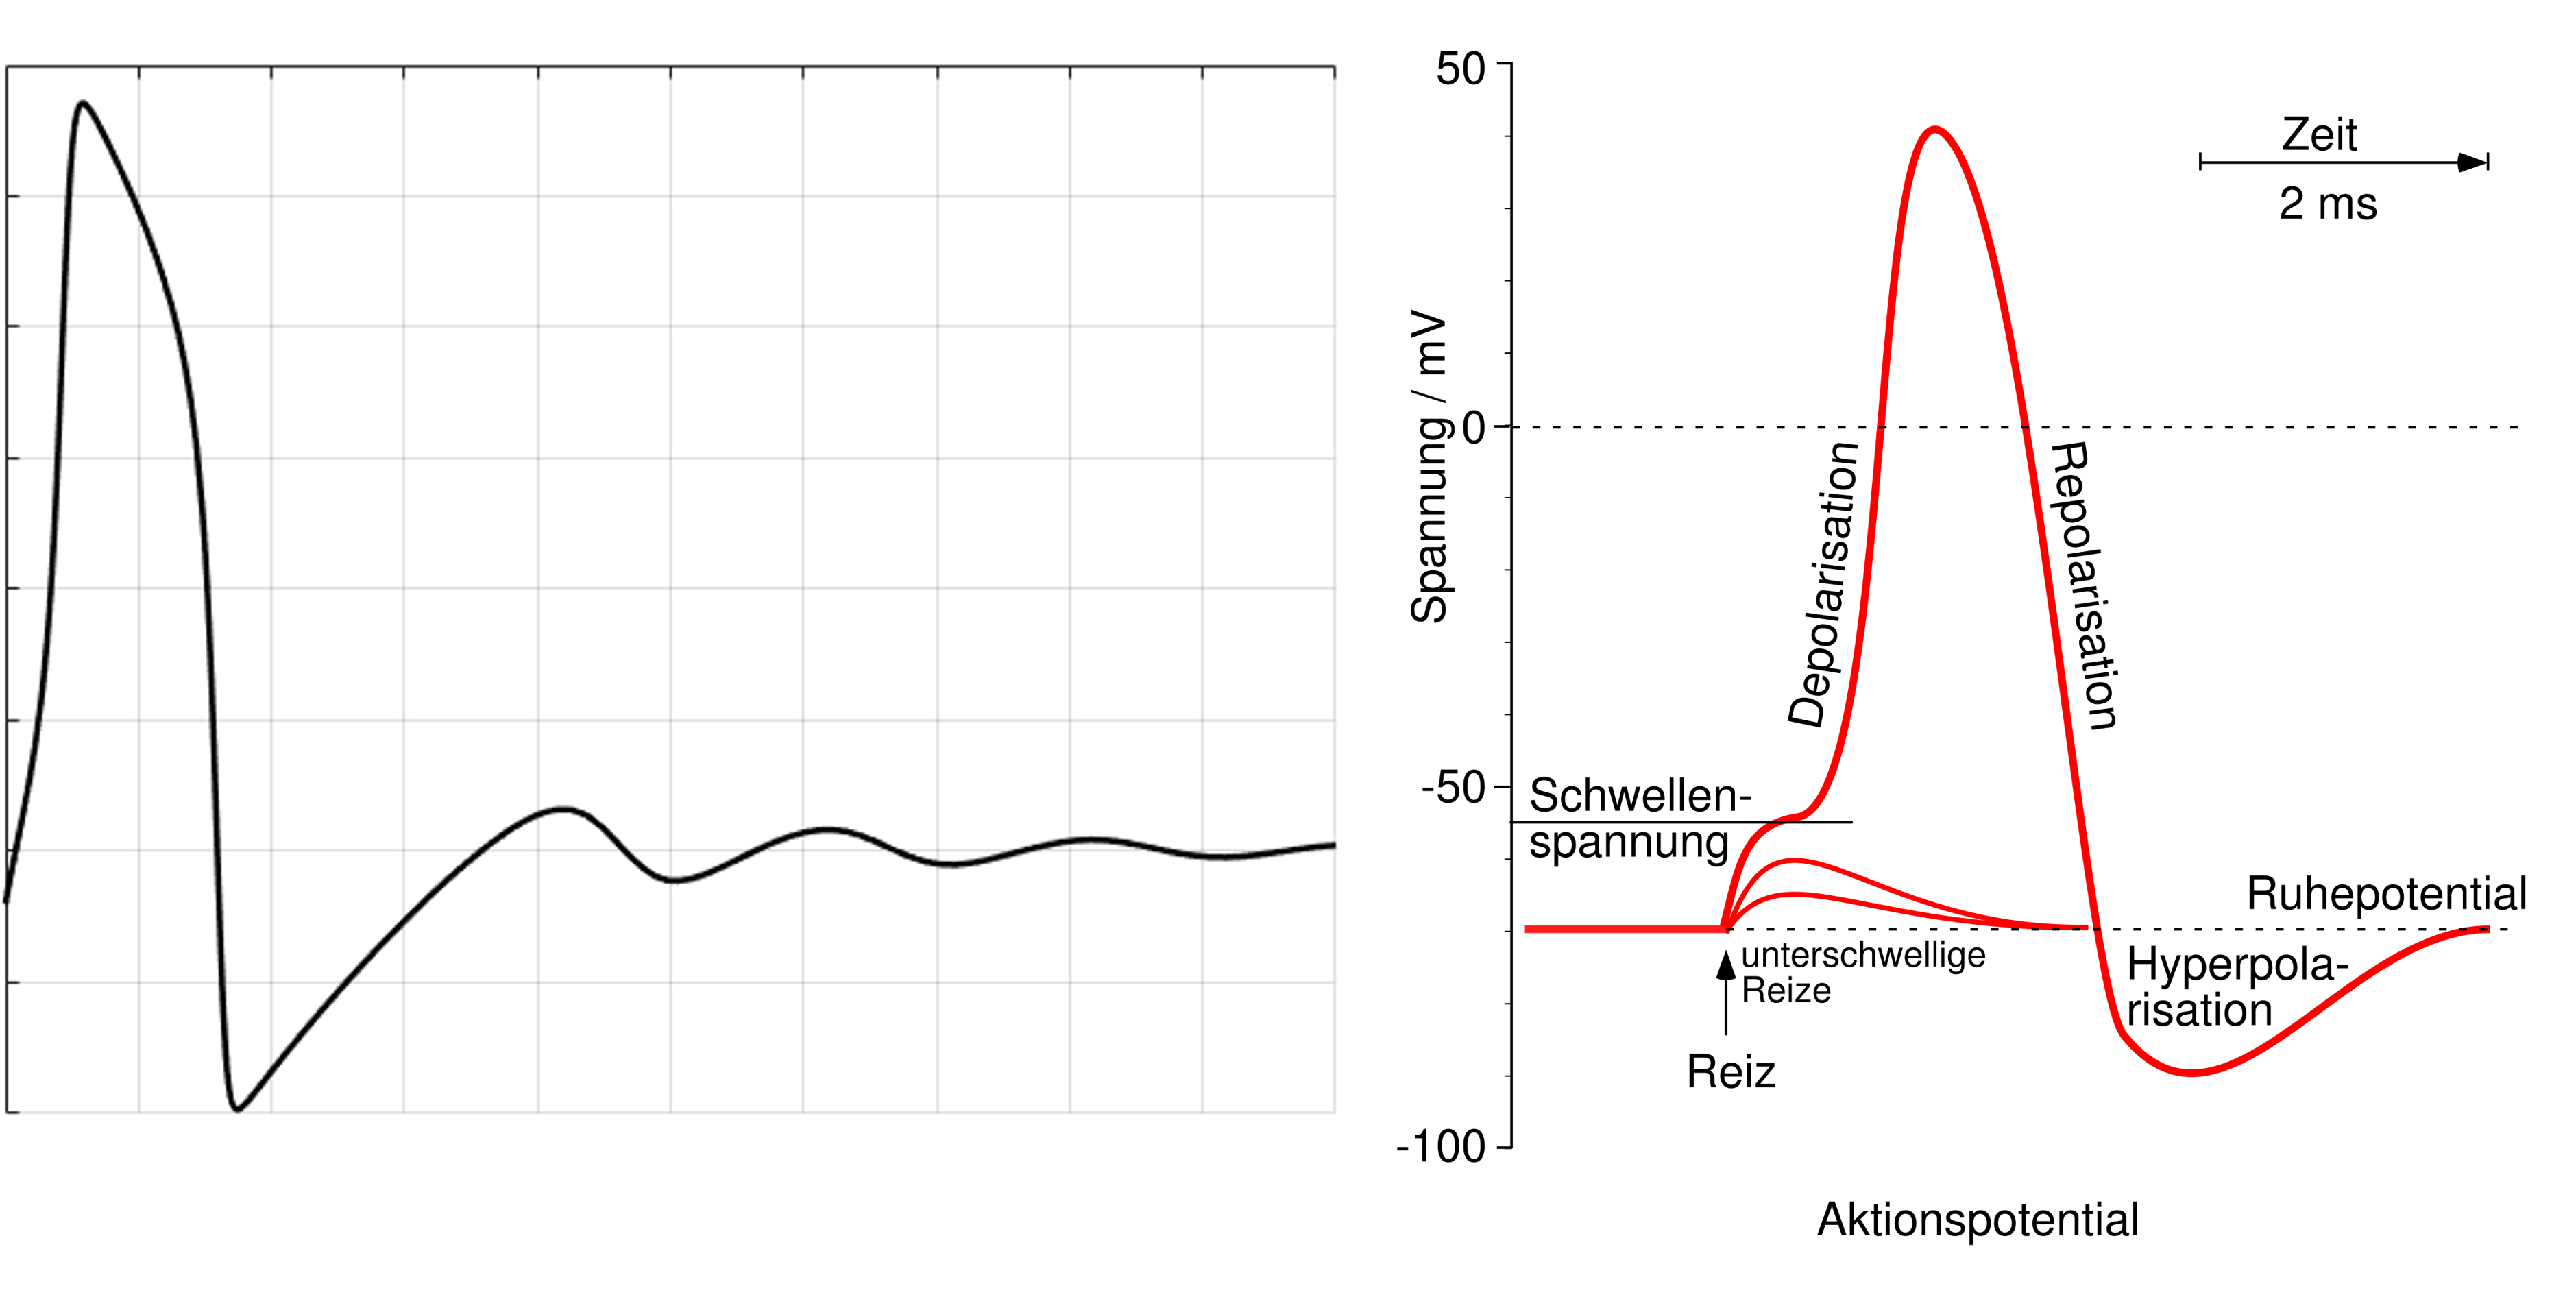
\includegraphics[width=\textwidth]{papers/nerven/Bilder/Vergleich.png}
    \caption{Vergleich $v$-Auslenkung Aktionspotential}
    \label{fig:Vergleich}
\end{figure}
\printbibliography[heading=subbibliography]
\end{refsection}